\documentclass[a4paper,12pt]{report}

\usepackage[T1]{fontenc}     % belső kódrendszer beállítása
\usepackage[utf8]{inputenc}  % input kódolás
\usepackage[magyar]{babel}   % nyelv
\usepackage{lmodern}


\usepackage{graphicx}
% \usepackage[center]{subfigure}
% \subfiglabelskip=0pt
\usepackage{subcaption }
\graphicspath{{./img/}}
\usepackage{amsmath}
\usepackage{amsfonts}
\usepackage{amssymb}
\usepackage{color}
\usepackage{hyperref}
\usepackage{anysize}
\usepackage{indentfirst}
\usepackage{amsthm}
\usepackage{mathtools}
\usepackage{titlesec}
\usepackage{bm}
\usepackage{enumitem}
\usepackage{nameref} 

% listings
\usepackage[dvipsnames]{xcolor}
\usepackage{textcomp}
\usepackage{listingsutf8}
\lstset{inputencoding=utf8/latin1}

\usepackage[numbered, framed ]{mcode} % autolinebreaks %MatLab code
\newcommand{\matlabpath}{"./matlab}

\usepackage{tikz}
\usepackage{appendix}

% \usepackage[ final ]{pdfpages}


% \usepackage{wrapfig}
% \usepackage{sidecap}
% \usepackage{subfig}
% \usepackage{latexsym}

\pagestyle{plain}
\marginsize{3.5cm}{2.5cm}{2.5cm}{2.5cm}
\frenchspacing
\sloppy % http://www.cs.bme.hu/~egmont/latex/
\linespread{1.5}


\hypersetup{
  linkcolor  = red,
  citecolor  = blue,
  urlcolor   = blue,
  colorlinks = true,
}


\newtheorem{theorem}{Tétel}%[section]
\newtheorem{lemma}[theorem]{Lemma}
\newtheorem{statement}[theorem]{Állítás}
\newtheorem{corollary}[theorem]{Következmény}
\newtheorem{definition}[theorem]{Definíció}
\newtheorem{remark}[theorem]{Megjegyzés}
\newtheorem{example}[theorem]{Példa}
\newtheorem{Fel}[theorem]{Feladat}
\newenvironment{solution}{\noindent \textbf{Megoldás. }}{ $\clubsuit$}
% \newenvironment{proof}{\noindent \textbf{Bizonyítás. }}{ $\square$}

%\newcommand{\dif}{\mathrm{d}}
\newcommand{\R}{\mathbb{R}}
\newcommand{\Z}{\mathbb{Z}}

\newcommand{\dd}{\,\mathrm{d}}
\DeclareMathOperator{\Div}{div}
\DeclareMathOperator{\grad}{\nabla}
\DeclareMathOperator{\supp}{supp}

\newcommand{\vr}[1]{\bm{#1}}
\newcommand{\mx}[1]{\bm{#1}}

% \newcommand{\overbar}[2][3]{{}\mkern#1mu\overline{\mkern-#1mu#2}}
\newcommand{\overbar}[1]{\mkern 1.5mu\overline{\mkern-1.5mu#1\mkern-1.5mu}\mkern 1.5mu}
\newcommand{\closure}[1]{\overbar{#1}}
\newcommand{\interior}[1]{\mathring{#1}}

\title{Diszkrét maximum-elv végeselem-módszerre elliptikus parciális differenciálegyenleteken}
\author{Balla Réka}
\date{\today}

\newenvironment{todo}{ \color{BurntOrange} \textbf{TODO}: \ }{}



\begin{document}

\titleformat{\chapter}
  {\normalfont\LARGE\bfseries}{\thechapter.}{1em}{}
\titlespacing*{\chapter}{0pt}{3.5ex plus 1ex minus .2ex}{2.3ex plus .2ex}

\thispagestyle{empty}
% \maketitle
\begin{center}


\begin{figure}[t]
\centerline{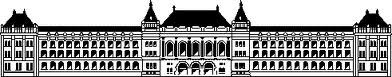
\includegraphics[ width=0.6\textwidth]{bmelogo.png}}
\end{figure}
\textbf{\small{Budapesti Műszaki és Gazdaságtudományi Egyetem\\Matematika Intézet}\\}
\vspace{2cm}

\textbf{\Large {SZAKDOLGOZAT\\}}
\vspace{1 cm}
 \textbf{\Large{Diszkrét maximum-elv végeselem-módszerre\\elliptikus parciális differenciálegyenleteken\\}}
  \vspace{1cm}														
  \textbf{\Large{Balla Réka}\\}
\vspace{3cm}

\begin{tabular}{rcl}  
\textbf{\large{Konzulens:}} & \hspace{1 cm} & \textbf{\large{Karátson János}}\\
  &   & \large{egyetemi tanár,}\\
  &   & \normalsize{ELTE TTK, Alkalmazott Analízis}\\
  &   & \normalsize{és Számításmatematika Tanszék,}\\  
  &   & \normalsize{BME, Analízis Tanszék}
\end{tabular}
 

 
 \vspace{2 cm}
\textbf{\Large{2017}}

\end{center}

\newpage

\thispagestyle{empty}
\input{Kivonat.tex}

\newpage

\pagenumbering{roman}

\tableofcontents

\newpage
\pagenumbering{arabic}




\chapter*{Bevezetés}
\addcontentsline{toc}{chapter}{Bevezetés}  


Valós folyamatok matematikai modellezésekor szeretnénk a valóságot minél jobban megközelíteni. A modell és modellezett folyamat közötti különbségeket általában két szempont szerint szokás vizsgálni: a kvantitatív (mennyiségi) vizsgálat a valós folyamat és a modell eredménye közötti eltérésre kíváncsi, a kvalitatív (minőségi) vizsgálat pedig a valós folyamatra jellemző tulajdonságok (pl. nemnegativitás vagy folytonosság) megmaradását  ellenőrzi. Ebben a dolgozatban az utóbbiról lesz szó. 
  
A parciális differenciálegyenletekkel leírható folyamatokhoz kapcsolódó legfontosabb kvalitatív tulajdonságok a  maximum-elvek, illetve azok következményei. Ezek közül is  leglényegesebb  a nemnegativitási tulajdonság, ugyanis sok olyan fizikai mennyiség van, ami nem vehet fel negatív értéket (pl. hőmérséklet Kelvinben, sűrűség), és ezt a tulajdonságot szeretnénk a folytonos matematikai modellre is átörökíteni. Mivel a legtöbb differenciálegyenlet csak numerikusan oldható meg, a numerikus modellektől is elvárjuk a folytonos modell kvalitatív tulajdonságaival ekvivalens tulajdonságok teljesülését.

A természetben előforduló fizikai jelenségek matematikai modelljei sok esetben vezetnek elliptikus parciális differenciálegyenletekre. Ilyenek például az energia típusú mennyiségek minimalizálási feladatai, vagy a folytonos közeg áramlását leíró egyensúlyi egyenletek. Ezeknek fontos jellemzőjük, hogy időfüggetlenek, így a numerikus megoldási módszereik alapvetően különböznek a parabolikus vagy hiperbolikus parciális differenciálegyenletekre alkalmazható numerikus módszerektől.

A dolgozatban a lineáris másodrendű elliptikus feladatokkal foglalkozunk, Dirichlet-peremfeltétel mellett. Tekintsük  $\Omega$ korlátos tartományon az
\begin{equation*}
	Lu = -\Div\left(p \nabla u \right) + q u
\end{equation*}
operátort, ahol $p \in C^1(\bar{\Omega})$, $q \in C(\bar{\Omega})$, $ 0 < p(x) $ és  $ 0 \leq q(x) $ teljesül $(\forall x \in \Omega)$. A Dirichlet-feladat ekkor $g \in C(\partial\Omega)$ esetén: keressük azt  $u \in C^2(\Omega) \bigcap C(\closure{\Omega})$ függvényt, amelyre:
\begin{equation*}	
	\left\{
	\begin{aligned}
		Lu &= f && \Omega \text{-ban}, \\
		u &= g & &\partial\Omega \text{-n}.
	\end{aligned}
	\right.
\end{equation*}



\Aref{ch:elmelet}. fejezetben ismertetjük a fentebb definiált Dirichlet-feladat végeselemes diszkretizációjának elméleti alapjait. Ehhez megfogalmazzuk  a $H^1(\Omega)$ Szoboljev-téren a gyenge feladatot, és összefoglaljuk a feladat megoldhatóságához kapcsolódó eredményeket. Ezután rátérünk a gyenge feladat végeselemes közelítésére, és bemutatjuk a Garjorkin-módszerrel  egy $W_h \subset H^1(\Omega)$  véges dimenziós altérre redukált feladatot. A redukált feladatban az eredeti feladat megoldásának azt az $u_h \in W_h$  közelítését keressük, amelyre
\begin{equation*}
	\begin{aligned}
		\int_{\Omega} \left( p \grad u_h \cdot \grad v_h + q u_h v_h \right) &= \int_{\Omega} f v_h,  \qquad (\forall v_h \in V_h ), \\
		u_h-\tilde{g}_h &\in V_h ,
	\end{aligned}
\end{equation*}
ahol  $V_h = W_h \cap H_0^1(\Omega)$ és $\tilde{g}|_{\partial\Omega} = g$ nyom értelemben, és $\tilde{g}_h$ a $\tilde{g}$ függvény  $W_h$-beli közelítése. Végül ismertetjük a végeselem-terekhez kapcsolódó fontosabb alapfogalmakat.

Ezután \aref{ch:Maxelvek}. fejezetben rátérünk a maximum-elvekre. Először a folytonos maximum-elvet mutatom be annak következményeivel, majd kimondom a klasszikus diszkrét maximum-elvet, ami nempozitív $f \in L^2(\Omega)$ forrásfüggvények esetén a következő tulajdonságokat feltételezi az $u_h$ közelítő megoldásra:
	\begin{equation*}
		\max_{\closure{\Omega}} u_h \leq \max \{0, \max_{\partial\Omega} g_h\},
	\end{equation*}
	emellett, ha $q \equiv 0$, akkor
	\begin{equation*}
		\max_{\closure{\Omega}} u_h =  \max_{\partial\Omega} g_h,
	\end{equation*}
ahol $g_h$ a $g$ peremfeltétel $W_h$-beli polinomiális interpolációja. Ezután mutatunk a végeselemes rácsra vonatkozó elégséges tulajdonságot a klasszikus diszkrét maximum-elv teljesülésére lineáris végeselemes approximáció esetén. Az utolsó szakaszban az 1 dimenziós Poisson-egyenletet vizsgáljuk homogén Dirichlet-peremmel, és mutatunk  ellenpéldát a klasszikus diszkrét maximum-elv kiterjesztésére a magasabbrendű közelítések esetére. A példát elemezve megfogalmazzuk az általános diszkrét maximum-elvet a vizsgált feladatra. Ennek lényege, hogy az $f$ forrásfüggvény nempozitivitása helyett az $f_h \in V_h$ nempozitivitását tesszük fel, ahol $f_h$ az $f$ függvény $V_h$ végeselemes altérre vett $L^2$-vetülete. A dolgozatban az általános diszkrét maximum-elvet csak a speciális alakú nempozitivitási, illetve nemnegativitási elvként fogalmazzuk meg: $\forall f_h \leq 0$ esetén az $u_h \in V_h \subset H_0^1(\Omega)$ közelítő megoldásra 
\begin{equation*}
	\max_{\closure{\Omega}} u_h \leq 0
\end{equation*}	
teljesül. Az általános diszkrét maximum-elv teljesülésére mutatható elégséges feltétel magasabbrendű végeselemes közelítésekre is.

 Végezetül \aref{ch:futtatas}. fejezetben egy konkrét példán keresztül mutatom be a klasszikus diszkrét maximum-elv teljesülését, és megvizgálom, hogy a forrásfüggvény változtatása hogyan befolyásolja az $u_h$ megoldás $0$-tól való eltérését. 

 

\chapter{Elméleti alapok}\label{ch:elmelet}


A dolgozatban másodrendű lineáris egyenletekkel foglalkozunk, a feladatokban Dirichlet-peremfeltételt alkamazva. Ebben a fejezetben \aref{sec:elliptikus}. részben ismertetjük az elliptikus feladatok megoldásához kapcsolódó alapfogalmakat, majd \aref{sec:fem}. szakaszban rátérünk a végeselemes közelítés elméleti alapjaira.


\section{Elliptikus feladatok megoldhatósága}\label{sec:elliptikus}


A végeselem-módszer elméleti alapjainál a gyenge megoldás fogalmára és a Szoboljev-térbeli becslésekre támaszkodunk, ezért ebben a részben röviden ismertetjük  a Szoboljev-tereket, majd rátérünk a gyenge feladat fogalmára, és igazoljuk ennek megoldhatóságát bizonyos feltételek mellett. Az itt leírtak legtöbbször \acite{pdnm, besenyei} jegyzeteket követik. 


Legyen $L$ a következő $\Omega$ korlátos tartományon értelmezett lineáris másodrendű elliptikus operátor:
\begin{equation}\label{L_op}
	Lu = -\Div\left(p \nabla u \right) + q u,
\end{equation}
ahol $p \in C^1(\bar{\Omega})$, $q \in C(\bar{\Omega})$, $ 0 < p(x) $ és  $ 0 \leq q(x) $ teljesül $(\forall x \in \Omega)$, és $u$ megfelelően sima függvény.  A továbbiakban feltesszük, hogy $\Omega \subset \R^d$, $d \geq 2$ és a $\partial\Omega$ perem szakaszonként sima és Lipschitz-folytonos.

Az $L$ operátorra megfogalmazható a Dirichlet-feladat:
\begin{definition}
Legyen $g \in C(\partial\Omega)$. Keressük azt  $u \in C^2(\Omega) \bigcap C(\closure{\Omega})$ függvényt, amelyre:
	\begin{equation}\label{dirichlet_problem}		
		\left\{
		\begin{aligned}
			Lu &= f && \Omega \text{-ban}, \\
			u &= g & &\partial\Omega \text{-n}.
		\end{aligned}
		\right.
	\end{equation}
	 Ha $g \equiv 0$ az $\Omega$ tartományon, akkor a feladatot homogénnek nevezzük, különben inhomogén feladatról beszélünk.
\end{definition}


\subsection{Szoboljev-terek}

Először definiáljuk a $H^1(\Omega)$ és  $H^1_0(\Omega)$ Szoboljev-tereket, majd röviden ismertetjük a később felhasznált állításokat, bizonyítások nélkül. Az állítások bizonyításai és a Szoboljev-terek részletesebb bemutatása megtalálhatók a \cite{besenyei} könyvben.

\begin{definition}
	Azt mondjuk, hogy  $u \in H^1(\Omega)$, ha $u \in L^2(\Omega)$, és ha léteznek olyan $g_1, \ldots, g_d \in L^2(\Omega)$ függvények, hogy 
	\begin{equation*}
		\int_{\Omega} u  \, \partial_i \varphi = - \int_{\Omega} g_i \, \varphi ,
	\end{equation*}
	minden $\varphi \in C_0^{\infty}(\Omega)$ és $i = 1, \ldots, d$ esetén.
	Ekkor az $u$ általánosított első parciális deriváltjait és gradiensét definiálhatjuk a következő képletekkel: 
	\begin{align*}
		\partial_i u &\coloneqq g_i, &
		\grad u &\coloneqq  (\partial_i u, \ldots, \partial_i).
	\end{align*}
	A $H^1(\Omega)$ téren a skalárszorzat és az indukált norma:
	\begin{align*}
		\langle u, v \rangle_{H^1(\Omega)} &\coloneqq \int_{\Omega} uv + \grad u \cdot \grad v,&  
		\| u \|_{H^1(\Omega)}^2 &\coloneqq \int_{\Omega} u^2 + |\grad u|^2.
	\end{align*}
\end{definition}


\begin{definition}
	Jelölje $H^1_0(\Omega)$ a $H^1$ tér megfelelő homogén peremfeltételt teljesítő alterét:
	\begin{equation*}
		H_0^1 \coloneqq \left\{u \in H^1(\Omega) : u|_{\partial\Omega} = 0 \right\},
	\end{equation*}
	ahol $ u|_{\partial\Omega}$ nyom-értelemben tekintendő. Ennek skalárszorzata a $H^1(\Omega)$-ból öröklődik.
\end{definition}


\begin{statement}
	A $H^1(\Omega)$ és  $H^1_0(\Omega)$ terek a megadott skalárszorzatra nézve Hilbert-terek.
\end{statement}

A Szoboljev-terek egyik alapvető becslése a következő egyenlőtlenség:

\begin{statement}[Poincaré-Friedrichs-egyenlőtlenség]\label{poin-fried}
	Van olyan $C_{\Omega} > 0$ konstans, hogy
	\begin{equation*}
		\| u \|_{L^2(\Omega)} \leq C_{\Omega} \| \grad u \|_{L^2(\Omega)} \quad (\forall u \in H^1_0(\Omega)),
	\end{equation*}
	azaz
	\begin{equation*}
		\int_{\Omega} u^2 \leq  C_{\Omega} \int_{\Omega} | \grad u |^2.
	\end{equation*}
\end{statement}
	

\begin{corollary}
	Az egyenlőtlenségből adódóan $H_0^1(\Omega)$-n a $H^1(\Omega)$-ból öröklöttel ekvivalens normát definiálhatunk:
	\begin{equation*}
		\| u \|_{H^1_0(\Omega)}^2 \coloneqq  \| \grad u \|_{L^2(\Omega)}^2 = \int_{\Omega} |\grad u|^2.
	\end{equation*}
	 Az ehhez tartozó skaláris szorzat:
	\begin{equation*}
		\langle u, v \rangle_{H^1_0(\Omega)} \coloneqq \int_{\Omega}  \grad u \cdot \grad v.
	\end{equation*}
	 A normák ekvivalenciája miatt $H_0^1(\Omega)$ az új skalárszorzatra nézve is Hilbert-tér.
\end{corollary}



\subsection{Gyenge feladat és megoldhatósága}

A gyenge megoldás fogalmához tekintsük \aref({dirichlet_problem})  feladat homogén esetét. Alakítsuk át a feladatot úgy, hogy az  $Lu = f$ egyenletet szorozzuk egy  $v \in (H_0^1(\Omega)$ függvénnyel, és vegyük az integrálját $\Omega$-n, a kapott egyenletre pedig alkalmazzuk a Green-formulát. Az így kapott feladat értelmes akkor is, ha $H^1_0(\Omega)$-n keressük a megoldást. Ezek alapján megfogalmazható a gyenge homogén Dirichlet-feladat:

\begin{definition}
	 Azt mondjuk, hogy \aref({dirichlet_problem}) Dirichlet-feladat homogén esetének gyenge megoldása  az $u\in H^1_0(\Omega)$ függvény, ha teljesül a következő egyenlőség: 
	\begin{equation}\label{gyenge_fealdat}
		\int_{\Omega} \left( p \grad u \cdot \grad v + q u v \right) = \int_{\Omega} f v  \qquad (\forall v \in H^1_0(\Omega)).
	\end{equation} 
\end{definition}

\begin{remark}\label{inhomogen}
	Az inhomogén eset visszavezethető homogén esetre. Tekintsük \aref({dirichlet_problem}) inhomogén Dirichlet-feladatot és legyen $\tilde{g} \in H^1(\Omega)$, melyre $\tilde{g}|_{\partial\Omega} = g$ nyom értelemben. Ekkor a homogén segédfeladat gyenge alakja felírható a $z \coloneqq u-\tilde{g}$ függvényre, ahol $u$ az eredeti inhomogén feladat gyenge megoldása:
	\begin{equation*}
		\int_{\Omega} \left( p \grad z  \cdot  \grad v + q z v \right) = \int_{\Omega} \left( f v - p \grad \tilde{g}  \cdot  \grad v - q \tilde{g} v \right) \qquad (\forall v \in H^1_0(\Omega)).
	\end{equation*}
	Ha ebben a jobb oldali $\tilde{g}$-os tagokat balra rendezzük, megkapjuk \aref({dirichlet_problem}) inhomogén Dirichlet-feladat szokásos gyenge alakját: keressük azt az $u \in H^1(\Omega)$ függvényt, amelyre
	\begin{equation*}
		\int_{\Omega} \left( p \grad u \cdot \grad v + q u v \right) = \int_{\Omega} f v  \qquad (\forall v \in H^1_0(\Omega)), 
	\end{equation*} 
	és $u|_{\partial\Omega}=g$ nyom értelemben, azaz $u-\tilde{g} \in H^1_0(\Omega)$. A tesztfüggvények itt is homogén peremfeltételt teljesítenek, mint a homogén feladat esetében.
\end{remark}



A gyenge megoldás létezése és egyértelműsége a Hilbert-térbeli bilineáris formák segítségével a Lax-Milgram elmélettel igazolható. A következő tétel  bizonyítása megtalálható a \cite{numfunk} jegyzet II.7.2. részében.

\begin{theorem}[Lax-Milgram-lemma]\label{lax-milgram}
	Legyen $H$ valós Hilbert-tér, $a: H \times H \rightarrow \R$ korlátos (folytonos), koercív bilineáris forma, azaz tegyük fel, hogy $\exists M > 0$ és $m > 0$, melyre $|a(u,v)| \leq M \|u\|\|v\|$ és $a(u,u) \geq m \|u\|^2$ $(\forall u, v \in H)$. Ekkor bármely $l : H \rightarrow \R$ korlátos lineáris funkcionálhoz létezik egyetlen olyan $u \in H$, melyre
	\begin{equation}\label{bilin_funk}
		a(u,v) = l(v) \qquad (\forall v \in H).
	\end{equation}
\end{theorem}



\Aref({gyenge_fealdat}) gyenge alakú feladat \aref({bilin_funk}) egyenlőség speciális esete:
\begin{align}\label{variacio_funk}
		a(u,v) &\coloneqq \int_{\Omega} (p \grad u \cdot \grad v + q u v)  ,&  l(v) &\coloneqq \int_{\Omega} f v,&  & u, v \in H^1_0(\Omega).		
\end{align}


Ha $p$ és $q$ függvények korlátosak, akkor az $a(u,v)$ bilineáris forma koercivitása és korlátossága a $p$ és $q$ függvények tulajdonságaiból adódnak.

\begin{statement}
	Legyen $p \in L^{\infty}(\Omega)$, $q \in L^{\infty}(\Omega)$ és $f \in L^2(\Omega)$. Ekkor \aref({gyenge_fealdat}) gyenge feladatnak létezik egyértelmű megoldása.
\end{statement}

\begin{proof}
	
	\Aref({variacio_funk})-ben definiált $a(u,v)$ formára teljesülnek \aref{lax-milgram} Lax-Milgram-lemma feltételei:
	\begin{itemize}
		\item $H^1_0(\Omega)$ valós Hilbert-tér.
		\item A bilinearitás az integrálás tulajdonságaiból következik.
		\item A korlátosság $p$ és $q$ korlátosságából, \aref{poin-fried}. Poincaré-Friedrichs-egynlőtlenségből, valamint a Cauchy–Bunyakovszkij–Schwarz-egyenlőtlenségből adódik:
			\begin{align*}
				|a(u,v)| &= \left| \int_{\Omega} (p \grad u \cdot \grad v + q u v)\right| 
							\leq \left| \int_{\Omega}  p \grad u \cdot \grad v \right| + \left| \int_{\Omega}  q u v \right| \leq \\ 
						% &\leq \|p\|_{L^{\infty}(\Omega)} \left|\langle \grad u, \grad v \rangle_{L^2(\Omega)} \right| + \|q\|_{L^{\infty}(\Omega)} \left|\langle u, v \rangle_{L^2(\Omega)} \right| \leq \\
						&\leq \|p\|_{L^{\infty}(\Omega)} \| \grad u\|_{L^2(\Omega)} \| \grad v\|_{L^2(\Omega)} + \|q\|_{L^{\infty}(\Omega)} \underbrace{\| u\|_{L^2(\Omega)} \| v\|_{L^2(\Omega)} }_{\leq C_{\Omega}^2 \| \grad u\|_{L^2(\Omega)} \| \grad v\|_{L^2(\Omega)}} \leq\\
						&\leq \underbrace{(\|p\|_{L^{\infty}(\Omega)} + \|q\|_{L^{\infty}(\Omega)} C_{\Omega}^2)}_{M} \| \grad u\|_{H^1_0(\Omega)} \| \grad v\|_{H^1_0(\Omega)},
			\end{align*} 
			ahol $C_{\Omega}$ Poincaré-Friedrichs konstans.
		\item A koercivitás $p$ pozitivitása és $q$ nemnegativitása miatt teljesül. Mivel $p > 0$, és $\Omega$ korlátos, ezért $\exists m > 0 $, amelyre $p \geq m$. Ekkor:
			\begin{equation*}
				a(u,u) =  \int_{\Omega} (p |\grad u|^2 + q u^2) \geq m  \int_{\Omega} |\grad u|^2 = m  \cdot \|u\|_{H_0^1(\Omega)}^2.
			\end{equation*}
	\end{itemize}
	Továbbá az  $f \in L^2(\Omega)$ feltételből következik, hogy $l$ korlátos lineáris funkcionál.
	
\end{proof}

\begin{remark}\label{LM_alter}
	\Aref{lax-milgram}. tétel alkalmazható akkor is, ha a $H_0^1({\Omega})$ Hilbert-tér helyett annak alterét tekintjük. Ezért ha \aref({gyenge_fealdat}) gyenge feladatot megszorítjuk  $H_0^1({\Omega})$ egy alterére, akkor is létezik egyértelmű megoldás, hiszen a tétel kritériumai igazak minden $u, v \in H_0^1({\Omega})$ függvényre, így az altérbeli $u$ és $v$ függvényekre is.
\end{remark}

\begin{remark}\label{szimm}
	\Aref({variacio_funk})-ben definiált $a(u,v)$ bilineáris forma szimmetrikus is, szintén az integrálás tulajdonságai miatt. Ez nem feltétele a Lax-Milgram-lemma teljesülésének, ezért a gyenge feladat nemszimmetrikus esetben is megoldható lenne.
\end{remark}


\section{A végeselem-módszer elméleti alapjai}\label{sec:fem}

A végeselem-módszer elméleti alapja a Galjorkin módszer. Ennek alapelve az, hogy \aref({gyenge_fealdat}) gyenge feladatot nem az egész $H_0^1(\Omega)$ téren próbáljuk megoldani, hanem ennek egy véges dimenziós  alterén. Ezt a közelítő megoldást az altér egy bázisának segítségével írjuk fel. Ha az alteret és annak bázisát úgy választjuk, hogy a báziselemek kis tartójú függvények legyenek, akkor a módszer megvalósítása lényegesen egyszerűbb lesz. További egyszerűsítés végett az alteret és annak bázisát legtöbbször úgy célszerű választani, hogy a bázisfüggvények szakaszonként polinomiálisak legyenek. Ekkor beszélhetünk végeselem-módszerről.

\subsection{A Galjorkin-módszer}


Legyen $V_h$ a $H_0^1(\Omega)$ Hilbert-tér egy $n$ dimenziós altere. Az alsó indexben szereplő $h>0$ paraméter a végeselem-módszernél a felosztás finomságát jellemzi majd. Ha \aref({gyenge_fealdat}) gyenge feladat megoldását a $u_h \in V_h$ függvények között keressük $V_h$-beli tesztfüggvények mellett, akkor a vetületi egyenlet:
\begin{equation}\label{vetuleti}
		a(u_h,v_h) = l(v_h) \qquad (\forall v \in V_h).
\end{equation}
Az egyenletre \aref{LM_alter}. megjegyzés szerint alkalmazható a Lax-Milgram-lemma, tehát van egyértelmű $u_h \in V_h$ megoldása. 

Az $u_h$ elemet a $V_h$ tér egy meghatározott $\{\varphi_1, \ldots, \varphi_n \}$ báziselemeinek lineáris kombinációjaként keressük:
\begin{equation}\label{linkomb}
		u_h = \sum_{j=1}^n c_j\varphi_j.
\end{equation}
\Aref({vetuleti}) vetületi egyenletben válasszuk tesztfüggvényeknek a $\varphi_i$ $(i = 1, \ldots , n) $ bázisfüggvényeket. Megmutatjuk, hogy így egyértelműen meghatározhatjuk a $c_j$ együtthatókat. Az egyenlet tehát:
\begin{equation*}
		a(u_h,\varphi_i) = l(\varphi_i) \qquad (i = 1, \ldots , n).
\end{equation*}
Az $a(u_h,\varphi_i)$ bilineáris formában $u_h$ helyére \eqref{linkomb} kifejezést helyettesítve a bilinearitás miatt kiemelhetjük a szummát és  a $c_j$ együtthatókat:
\begin{equation*}
		\sum_{j=1}^n a(\varphi_j,\varphi_i)c_j = l(\varphi_i) \qquad (i = 1, \ldots , n).
\end{equation*}
Ez egy  $n \times n$ méretű lineáris egyenletrendszer. Vezessük be az 
\begin{equation}\label{hom_matrixok}
	\begin{aligned}
		(\mx{A_h})_{ij} &\coloneqq a(\varphi_j,\varphi_i) \quad (i,j = 1, \ldots, n),\\ 
		\vr{b_h} &\coloneqq (l(\varphi_1),\ldots ,l(\varphi_n))^T, \\
		\vr{c_h} &\coloneqq (c_1, \ldots , c_n)^T
	\end{aligned}
\end{equation}
jelöléseket. Ekkor az egyenletrendszer mátrixos alakban:
\begin{equation}\label{lin_rsz}
	\mx{A_h}\vr{c_h} = \vr{b_h} .
\end{equation}

\begin{statement}\label{szimpoz}
	\Aref({lin_rsz}) lineáris egyenletrendszerben az $\mx{A_h}$ mátrix szimmetrikus és pozitív definit.
\end{statement}

\begin{proof}
	 A szimmetria  az  $a(.,.)$ bilineáris forma szimmetriájából (\ref{szimm} megjegyzés) közvetlenül következik.
	 
	 Legyenek  $u_h$ és $v_h$ tetszőleges $V_h$ -beli elemek. Írjuk fel ezeket a  $\{\varphi_1, \ldots, \varphi_n \}$ báziselemek lieáris kombinációjaként:
	\begin{equation*}
			u_h = \sum_{j=1}^n c_j\varphi_j, \qquad  v_h = \sum_{j=1}^n d_j\varphi_j,
	\end{equation*}
	és jelölje $\vr{c}, \vr{d} \in \R^n$ rendre a $c_j$ és $d_j$ együtthatók vektorait. Ekkor
	\begin{equation*}
			a(u_h,v_h) = a\left( \sum_{j=1}^n c_j\varphi_j, \sum_{j=1}^n d_j\varphi_j \right) = \sum_{i,j=1}^n a(\varphi_j,\varphi_i)c_j d_i = \mx{A_h}\vr{c} \cdot \vr{d}.
	\end{equation*}
	Ebböl $u_h = v_h$ esetben az $a(.,.)$ bilineáris forma koercivitása miatt:
	\begin{equation*}
			\mx{A_h}\vr{c} \cdot \vr{c} =  a(u_h,u_h) > 0,
	\end{equation*}
	tehát $\mx{A_h}$ pozitív definit.
\end{proof}

\begin{corollary}
	\Aref({lin_rsz}) lineáris egyenletrendszernek egyértelműen létezik $\vr{c_h} \in \R^n$ megoldása.
\end{corollary}

 Tehát \aref({dirichlet_problem})  feladat homogén változatának közelítő megoldása  Galjorkin-módszerrel az így kapott \eqref{lin_rsz} egyenletrendszer megoldása. Az $\mx{A_h}$ mátrix szokásos elnevezése merevségi mátrix (angolul 'stiffness matrix'), a jobb oldalon álló  $\vr{b_h}$ vektoré pedig tehervektor (angolul 'load vector'). A Galjorkin-módszer alkalmazható lenne akkor is, ha az $a$ bilineáris forma, és így merevségi mátrix nem lenne szimmetrikus.
 
 Az egyenletrendszer merevségi mátrixának és tehervektorának elemei tehát a következő képletekkel számíthatók:
\begin{gather*}
	(\mx{A_h})_{ij}  = a(\varphi_j,\varphi_i) = \int_{\Omega} (p \grad \varphi_j  \cdot  \grad \varphi_i + q \varphi_j \varphi_i), \quad  (i,j = 1, \ldots ,n),\\
	(\vr{b_h})_i =  l(\varphi_i) = \int_{\Omega} f \varphi_i, \quad (i = 1, \ldots ,n).
\end{gather*}
Ha  a $V_h$ altér $\{\varphi_1, \ldots, \varphi_n \}$ bázisát úgy választjuk meg, hogy a bázisfüggvények kis tartójúak legyenek, akkor a $\varphi_j,\varphi_i$ függvények tartói között kevés az átfedés, így az $a(\varphi_j,\varphi_i)$ elemek között sok nulla lesz.  A bázisfüggvények sorrendjének alkalmas megválasztásával az $\mx{A_h}$ mátrix sokszor sávmátrix lesz, ezért \aref({lin_rsz}) egyenletrendszer megoldása lényegesen egyszerűbbé válik. Ha ezen felül a bázisfüggvények még szakaszonként polinomiálisak is, akkor az $a(\varphi_j,\varphi_i)$ és $l(\varphi_i)$ értékek kiszámítása lesz könnyebb.

 
 Az inhomogén Dirichlet-feladat esetén a $V_h$ altér bázisát kell kibővítenünk. \Aref{inhomogen}. megjegyzésben láttuk az inhomogén feladat gyenge alakját: keressük azt az  $u \in H^1(\Omega)$ függvényt, amelyre
 \begin{equation*}
		\int_{\Omega} \left( p \grad u \cdot \grad v + q u v \right) = \int_{\Omega} f v  \qquad (\forall v \in H^1_0(\Omega)), 
\end{equation*} 
és $u$-ra teljesül továbbá, hogy
\begin{align*}
	&u|_{\partial\Omega}=g \quad \text{nyom értelemben} & &\Longleftrightarrow& &u-\tilde{g} \in H^1_0(\Omega).&
\end{align*}
A $v$ tesztfüggvények itt is homogén peremfeltételűek. 

A Galjorkin-módszerben az $u$  függvényt a $W_h \subset H^1(\Omega)$ altéren közelítjük. A tesztfüggvények tere legyen $V_h \coloneqq \{v \in W_h : v \in H_0^1(\Omega) \} $  altér. \Aref{inhomogen}. megjegyzésben bevezetett $\tilde{g}$ függvény $W_h$-beli közelítését jelölje $\tilde{g}_h$, a $z = u- \tilde{g}$ függvény $V_h$-beli vetületét pedig jelölje $z_h$.  A korábban bevezetett \eqref{variacio_funk} formákkal a Galjorkin-feladat: keressük azt az $u_h \in W_h$ függvényt a $\tilde{g}_h \in W_h$ vetületi peremfeltétel mellett, amelyre  teljesül az inhomogén vetületi egyenlet:
\begin{equation}\label{inhom_vetegy}
	\begin{aligned}
		a(u_h,v_h) &= l(v_h)  \qquad (\forall v \in V_h), \\
		u_h-\tilde{g}_h &\in V_h
	\end{aligned}
\end{equation}


A $W_h$ altérhez olyan bázist kell választanunk, amely homogén és inhomogén peremfeltételű tagokat is tartalmaz. A korábban bevezetett $\{\varphi_1, \ldots, \varphi_n \}$ jelölést megtartjuk a $V_h$-beli báziselemekre, és ehhez hozzávesszük a $\{\varphi_{n+1}, \ldots, \varphi_{n+m}\}$ inhomogén peremfeltételű, $W_h$-beli báziselemeket a perem közelítésére. Így az új bázis:
 \begin{equation*}
	\varphi_1, \ldots, \varphi_n,\varphi_{n+1}, \ldots, \varphi_{n+m},
 \end{equation*}
 és a közelítő megoldást a következő alakban keressük:
 \begin{equation*}
	u_h = \underbrace{\sum_{j=1}^n c_j\varphi_j }_{z_h}+ \underbrace{\sum_{j=n+1}^{n+m} c_j\varphi_j}_{\tilde{g}_h}.
 \end{equation*}

Általában a $\{\varphi_{n+1}, \ldots, \varphi_{n+m}\}$ inhomogén peremfeltételű báziselemeket úgy válsztjuk, hogy tartójuk a perempontok egy kis környezete legyen, így a szumma második része a $g$ peremfeltétel közelítésének tekinthető a peremen. Ekkor nincs szükség $\tilde{g}_h$ kiszámítására, a $c_{n+1}, \ldots, c_{n+m}$ együtthatók ismertnek tekinthetők, ezért ezekre bevezetjük rendre a $g_{1}, \ldots, g_{m}$ jelöléseket.

A mátrixos alak felírásához legyen
\begin{equation}\label{inhom_matrixok}
	\begin{aligned}
		(\mx{\tilde{A}_h})_{i,j} &\coloneqq a(\varphi_{n+j},\varphi_i) \quad (i = 1, \ldots, n, \, j = 1, \ldots, m),\\ 
		\vr{g_h} &\coloneqq (c_{n+1}, \ldots, c_{n+m})^T = (g_{1}, \ldots, g_{m})^T,
	\end{aligned}
\end{equation}
 és legyen $\mx{A_h}$, $\vr{c_h}$ és $\vr{b_h}$ ugyanaz, mint \aref({hom_matrixok}) pontban, homogén esetben. Ekkor az inhomogén feladatra az $n \times n$ méretű lineáris egyenletrendszer mátrixos alakja:
 \begin{equation}\label{inhom_ler}
	\mx{A_h}\vr{c_h} + \mx{\tilde{A}_h} \vr{g_h} = \vr{b_h}, 
 \end{equation}
ahol az ismeretlen $\vr{c_h} \in \R^n$ vektort keressük továbbra is. Az $\mx{A_h}$ mátrixra továbbra is érvényes \aref{szimpoz}. állítás, ezért létezik egyértelmű megoldás. Az egyenletrendszert átrendezhetjük egy $(n+m) \times (n+m)$ méretű bővített egyenletrendszerré. Vezessük be a következő jelöléseket: 
\begin{align}\label{inhom_mx_def}
	&\mx{\widehat{A}_h} \coloneqq 
		\begin{bmatrix}
			\mx{A_h} & \mx{\tilde{A}_h} \\
			\mx{0} & \mx{I}
		\end{bmatrix},&
	&\vr{\widehat{c}_h} \coloneqq 
		\begin{bmatrix}
			\vr{c_h} \\ 
			\vr{g_h}
		\end{bmatrix},& 
	&\vr{\widehat{b}_h} \coloneqq 
		\begin{bmatrix}
			\vr{b_h} \\
			\vr{g_h}
		\end{bmatrix},&
 \end{align}
ahol $\mx{0}$ az $m \times n$ méretű nullmátrix, $\mx{I}$ pedig az $m \times m$ méretű egységmátrix. A kibővített egyenletrendszer:
\begin{equation}\label{inhom_dirichlet_egyrendszer}
	\mx{\widehat{A}_h} \vr{\widehat{c}_h}  = \vr{\widehat{b}_h}.
 \end{equation}

 
% \begin{todo}

% \subsection{A Ritz-módszer}
% \begin{remark}
	
	% \Aref({dirichlet_problem}) feladatbeli egyenletre megfogalmazható a minimalizációs feladat is: keressük azt az $u \in H^1_0(\Omega)$ függvényt, ami minimalizálja az 
	% \begin{equation}\label{min_feladat}
		% I(u) = \frac{1}{2} \int_{\Omega} \left( p |\grad u|^2 + q u^2 - u f \right)
	% \end{equation}
	% funkcionált. Ugyanez \aref({variacio_funk}) jelöléssel:
	% \begin{equation}
		% I(u) = \frac{1}{2} \cdot a(u,u) - l(u)
	% \end{equation}
	
% \end{remark}


% \begin{remark}
	
	% \Aref({variacio_funk}) $a(u,v)$ bilineáris forma szimmetrikus, bilineáris, és a koercivitás miatt pozitív definit is. Ezek együttes következménye, hogy \aref({min_feladat}) feladat megoldása is egyértelmű, illetve hogy \aref({gyenge_fealdat}) és \aref({min_feladat}) feladatok megoldása megegyezik. Ez szintén igaz akkor is, ha a a feladatokban $H_0^1(\Omega)$ helyett annak zárt konvex részhalmazát tekintjük. 
% \end{remark}

% A minimalizációs feladatban definiált $I(u)$ funkcionál fizikai jelentése szerint a differenciálegyenlet által modellezett rendszer energiájét jellemző mennyiség, ezért a feladat megoldása az energiaminimum elvének érvényesítését jelenti.

% \end{todo}

 
\subsection{Végeselem-terek}

Láttuk, hogy a Galjorkin-módszer tényleges megvalósítása függ attól, hogy milyen $V_h$, vagy inhomogén esetben $W_h$ alteret, és milyen bázist választunk. A végeselem-módszerben ezek a bázisfüggvények általában ``szakaszonként'' polinomok, kis tartóval, a résztartományok $d$ dimenziós poliéderek, és a közelítő megoldást folytonosnak konstruáljuk az egész tartományon.

Feltesszük, hogy $\closure{\Omega}$ egy $\R^d$-beli poliéder, ekkor  a tartomány felbontását a következőképpen értelmezzük:

\begin{definition}
	Az $\Omega$ tartomány triangulációjának nevezzük a 
	\begin{equation*}
		\mathcal{T}_h \coloneqq \{ T_1, \ldots, T_M \}
	\end{equation*}
	halmazt, ahol
	\begin{enumerate}[label=(\roman*)]
		\item $\forall T_k \in \mathcal{T}_h $ az $\closure{\Omega}$ zárt részhalmaza, a belseje, $\interior{T_k}$ nemüres, és a peremen  Lipschitz-folytonos. A dolgozatban feltesszük, hogy ezek poliéderek.
		\item $\displaystyle  \bigcup_{k=1}^{M} T_k = \closure{\Omega}$,
		\item $\interior{T_i} \bigcap \interior{T_j} = \emptyset$, ha $i \neq j$,
		\item a felbontás konform, azaz $T_i \bigcap T_j$ ($i \neq j$) üres, vagy a közös, alacsonyabb, de azonos dimenziós lapja a $T_i, T_j$ elemeknek.
	\end{enumerate}
\end{definition}

\begin{definition}\label{def:finomság}
	A $\mathcal{T}_h$ trianguláció finomsága a fellépő legnagyobb átmérő:
	\begin{equation*}
		h \coloneqq \max_{1 \leq k \leq M} diam(T_k).		
	\end{equation*}
\end{definition}

A $W_h$ (vagy homogén esetben $V_h$) altér legyen olyan, hogy elemei ``szakaszonként'' polinomok és folytonosak az egész tartományon:
\begin{equation*}
	W_h \subset \left\{ u \in C(\closure{\Omega}): u|_{T_k} \in P^{l_k}, \forall T_k \in \mathcal{T}_h  \right\},
\end{equation*}
ahol $P^{l_k}$ jelöli a legfeljebb $l_k$-adfokú polinomok $T_k$-ra való megszorításainak halmazát.

Általában $W_h$-ra teljesülnek a következő tulajdonságok is:
\begin{itemize}
	\item A $T_k$ halmazok azonos típusúak pl. csak nem elfajuló $d$-szimplexek.
	\item $l_k \equiv l$, vagyis minden résztartományok azonos fokú polinomokat tekintünk.
	\item Előfordulhat, hogy $W_h$-ban $u|_{T_k}$ nem az összes legfeljebb $l_k$-adfokú polinomot veheti fel.
	\item Az $l$-edfokú polinomokat $T_k$-ban kijelölt csomóponti értékek határozzák meg. Ezek függvényértékek vagy deriváltértékek lehetnek. Amikor a csomóponti értékek csak függvényértékek, akkor a bázis olyan polinomokból áll, melyek egy adott csomópontban $1$-et, a többiben $0$-t vesznek fel, azaz, ha $x_1, \ldots, x_r$ jelöli a csomópontokat, akkor 
		\begin{equation*}
			\varphi(x_i) = \delta_{ij},
		\end{equation*}
		ahol $\delta_{ij}$ a Kronecker-szimbólum.
\end{itemize}


\begin{example}\label{1dpelda}
	1D-ben a legegyszerűbb $W_h$ altér a folytonos, szakaszonként lineáris függvények tere, melynek bázisát a $\varphi_i(x_j) = \delta_{i,j}$ kalapfüggévnyek alkotják (lásd \ref{fig:1dlinearis} ábra).
\end{example}

\begin{figure}[h!]
	\begin{subfigure}{\textwidth}
		\centerline{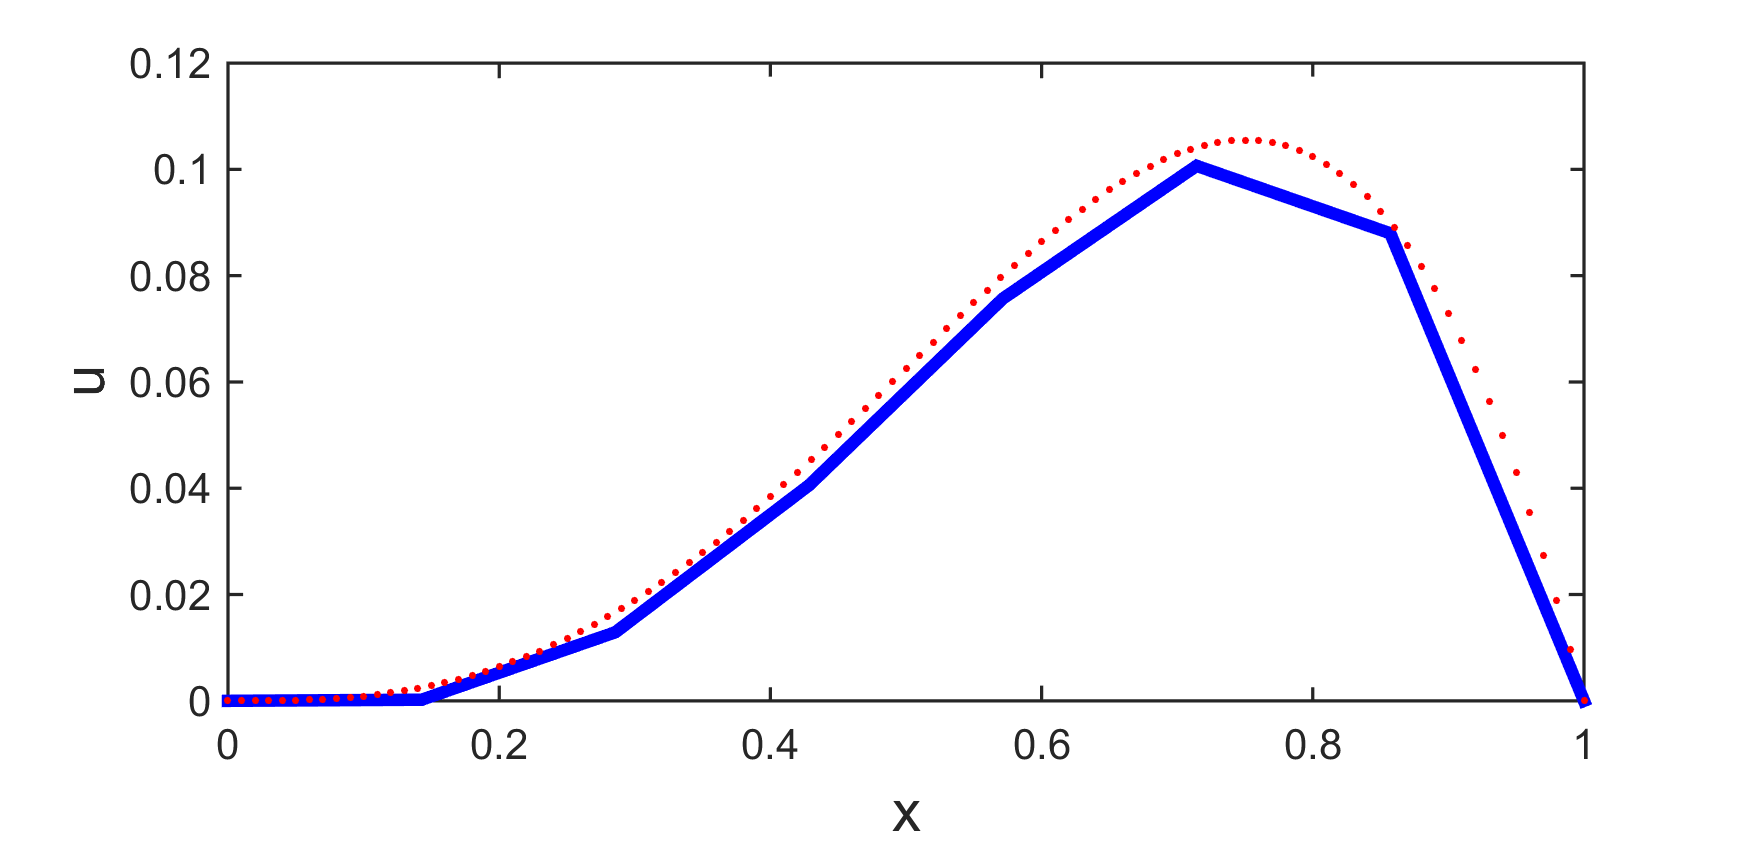
\includegraphics[width= .7\linewidth]{1dpelda.png}}
		\label{fig:linu1d}
	\end{subfigure}\\
	\begin{subfigure}{\textwidth}
		\centerline{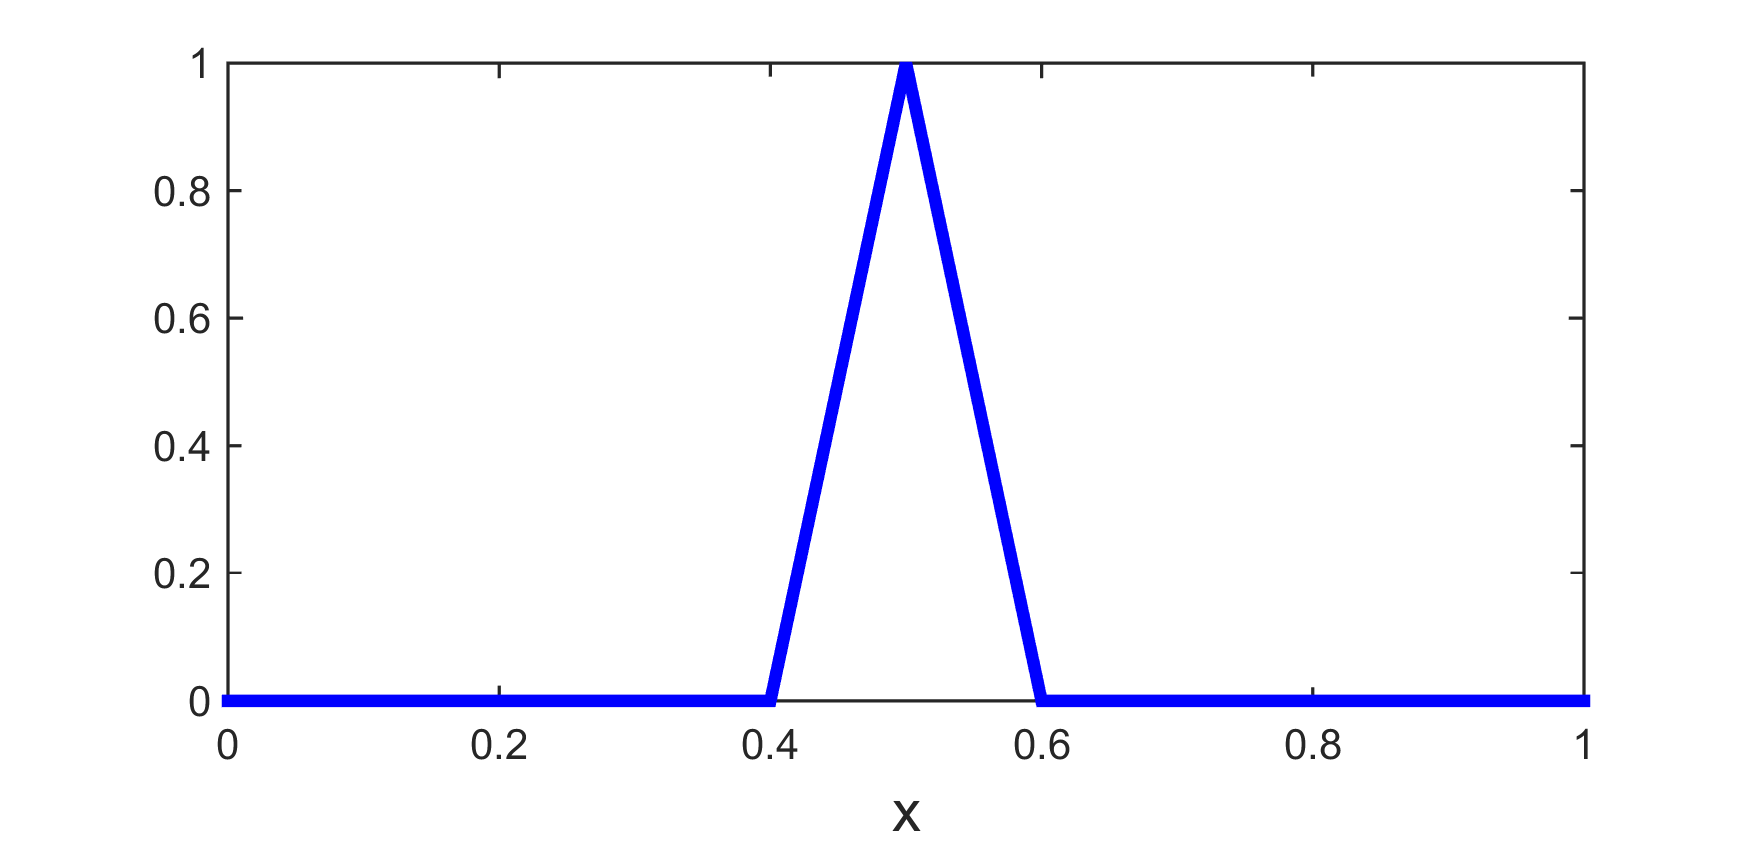
\includegraphics[width= .7\linewidth]{kalapfv.png}}
		\label{fig:sator1d}
	\end{subfigure}
	\caption{\Aref{1dpelda}. példa $W_h$ altere a $[0,1]$ intervallumon: $u_h$ szakaszonként lineáris (felső ábra), a báziselemek a $\phi_i(x_j) = \delta_{i,j}$ kalapfüggvények (alsó ábra)}
	\label{fig:1dlinearis}
\end{figure}
	
\begin{example}\label{2dpelda}
	2D-ben a leggyakrabban használt trianguláció $T_k$ elemei nem elfajuló háromszögek, $u|_{T_k}$ folytonos, szakaszonként lineáris függvény, és a csomóponti értékek a háromszög csúcsaiban vett függvényértékek. A $W_h$ altér:
	\begin{equation*}
		W_h = \left\{ u \in C(\closure{\Omega}): u|_{T_k} \in P^1, \forall T_k \in \mathcal{T}_h  \right\}.
	\end{equation*}
	Ezeknek a végeselemeknek szokásos elnevezése a $\mathbf{T_3}$ vagy Courant-elem. A $W_h$ altér bázisát (a síkbeli csomópontokat most $(x_i,y_j)$-vel jelölve) a $\varphi_{ij}(x_k,y_l) = \delta_{ik} \cdot \delta_{jl}$ feltétel alapján meghatározott sátorfüggvények alkotják.  A megoldás alakját és a báziselemeket a  \ref{fig:2dlinearis} ábra szemlélteti.
\end{example}

\begin{figure}[h!]
	\begin{subfigure}{\textwidth}
		\centerline{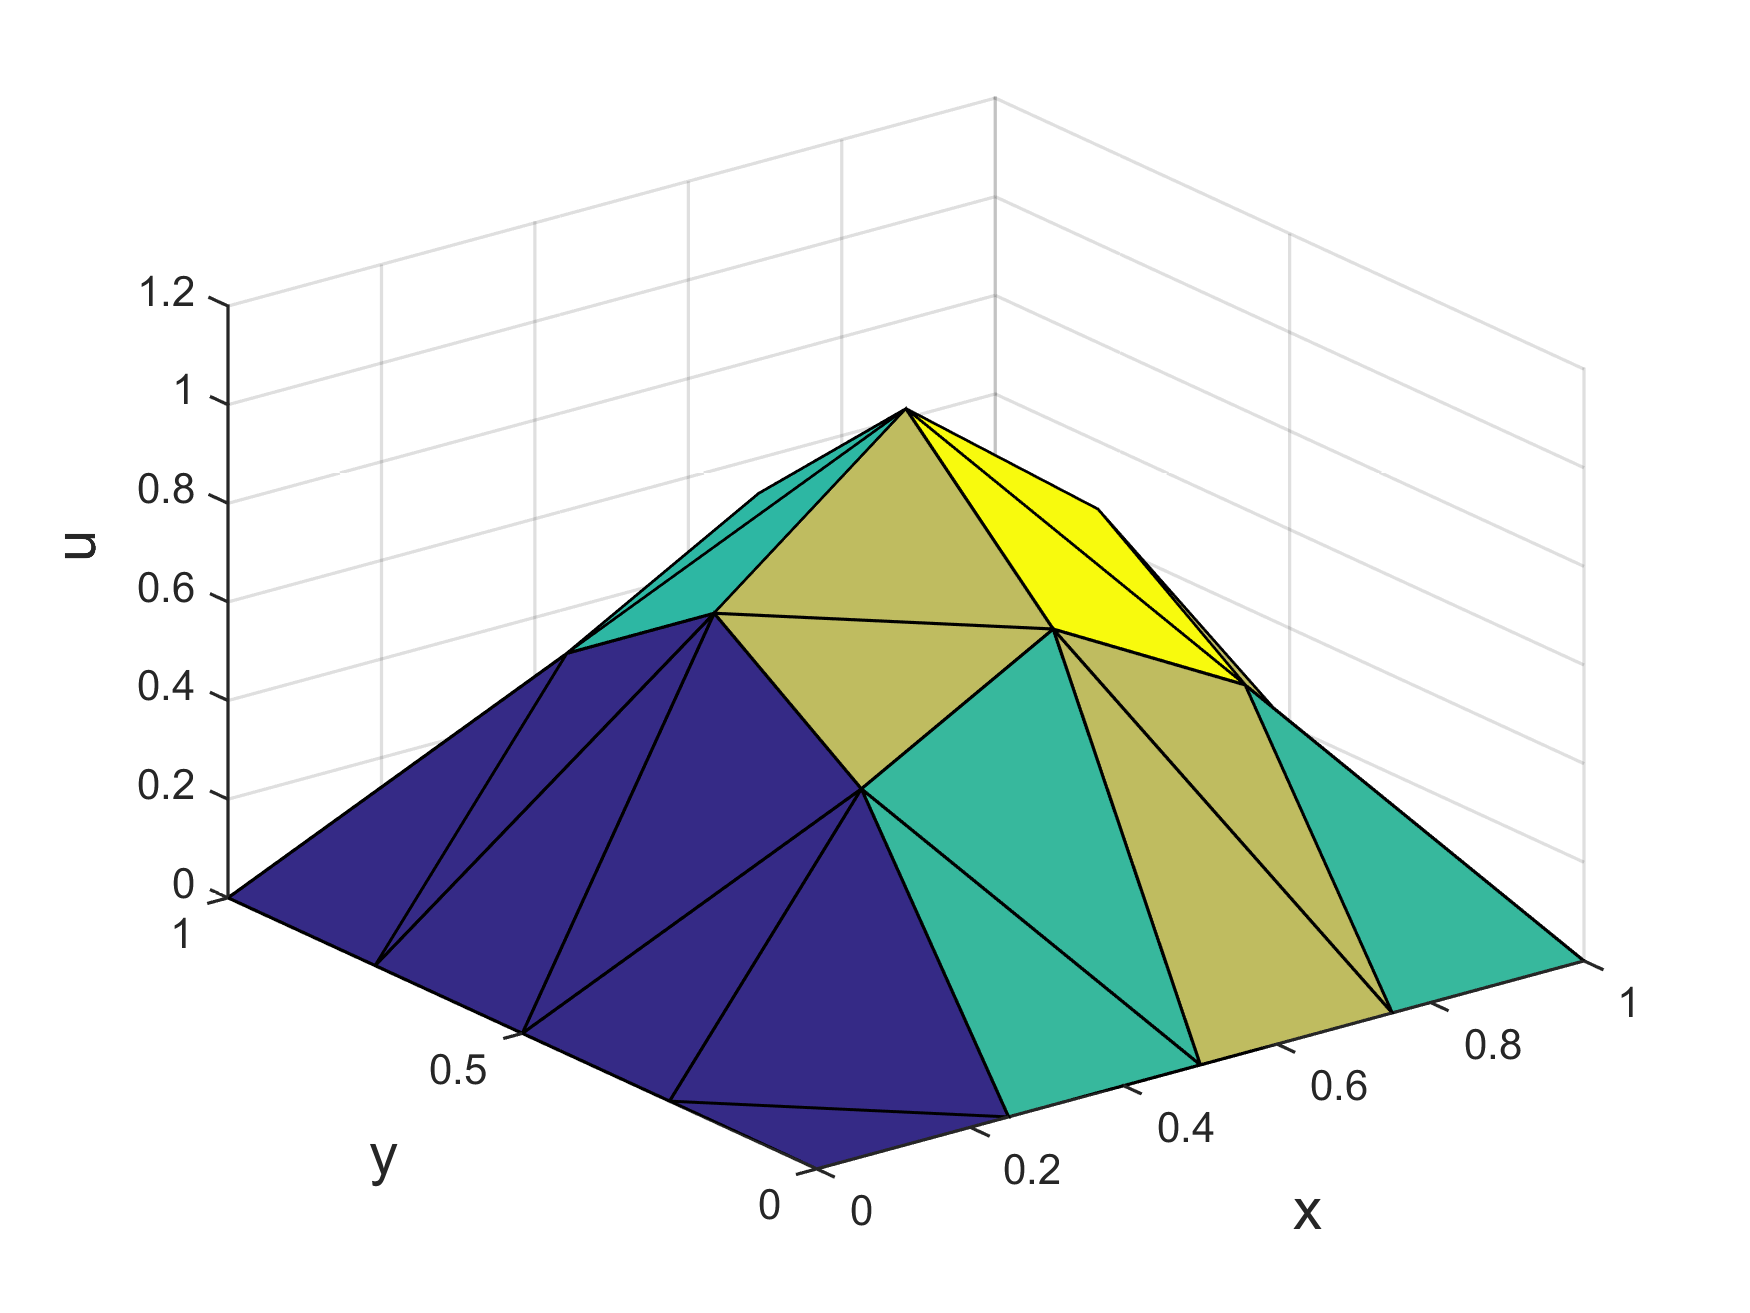
\includegraphics[width= .7\linewidth]{2dpelda.png}}
		\label{fig:linu2d}
	\end{subfigure}\\
	\begin{subfigure}{\textwidth}
		\centerline{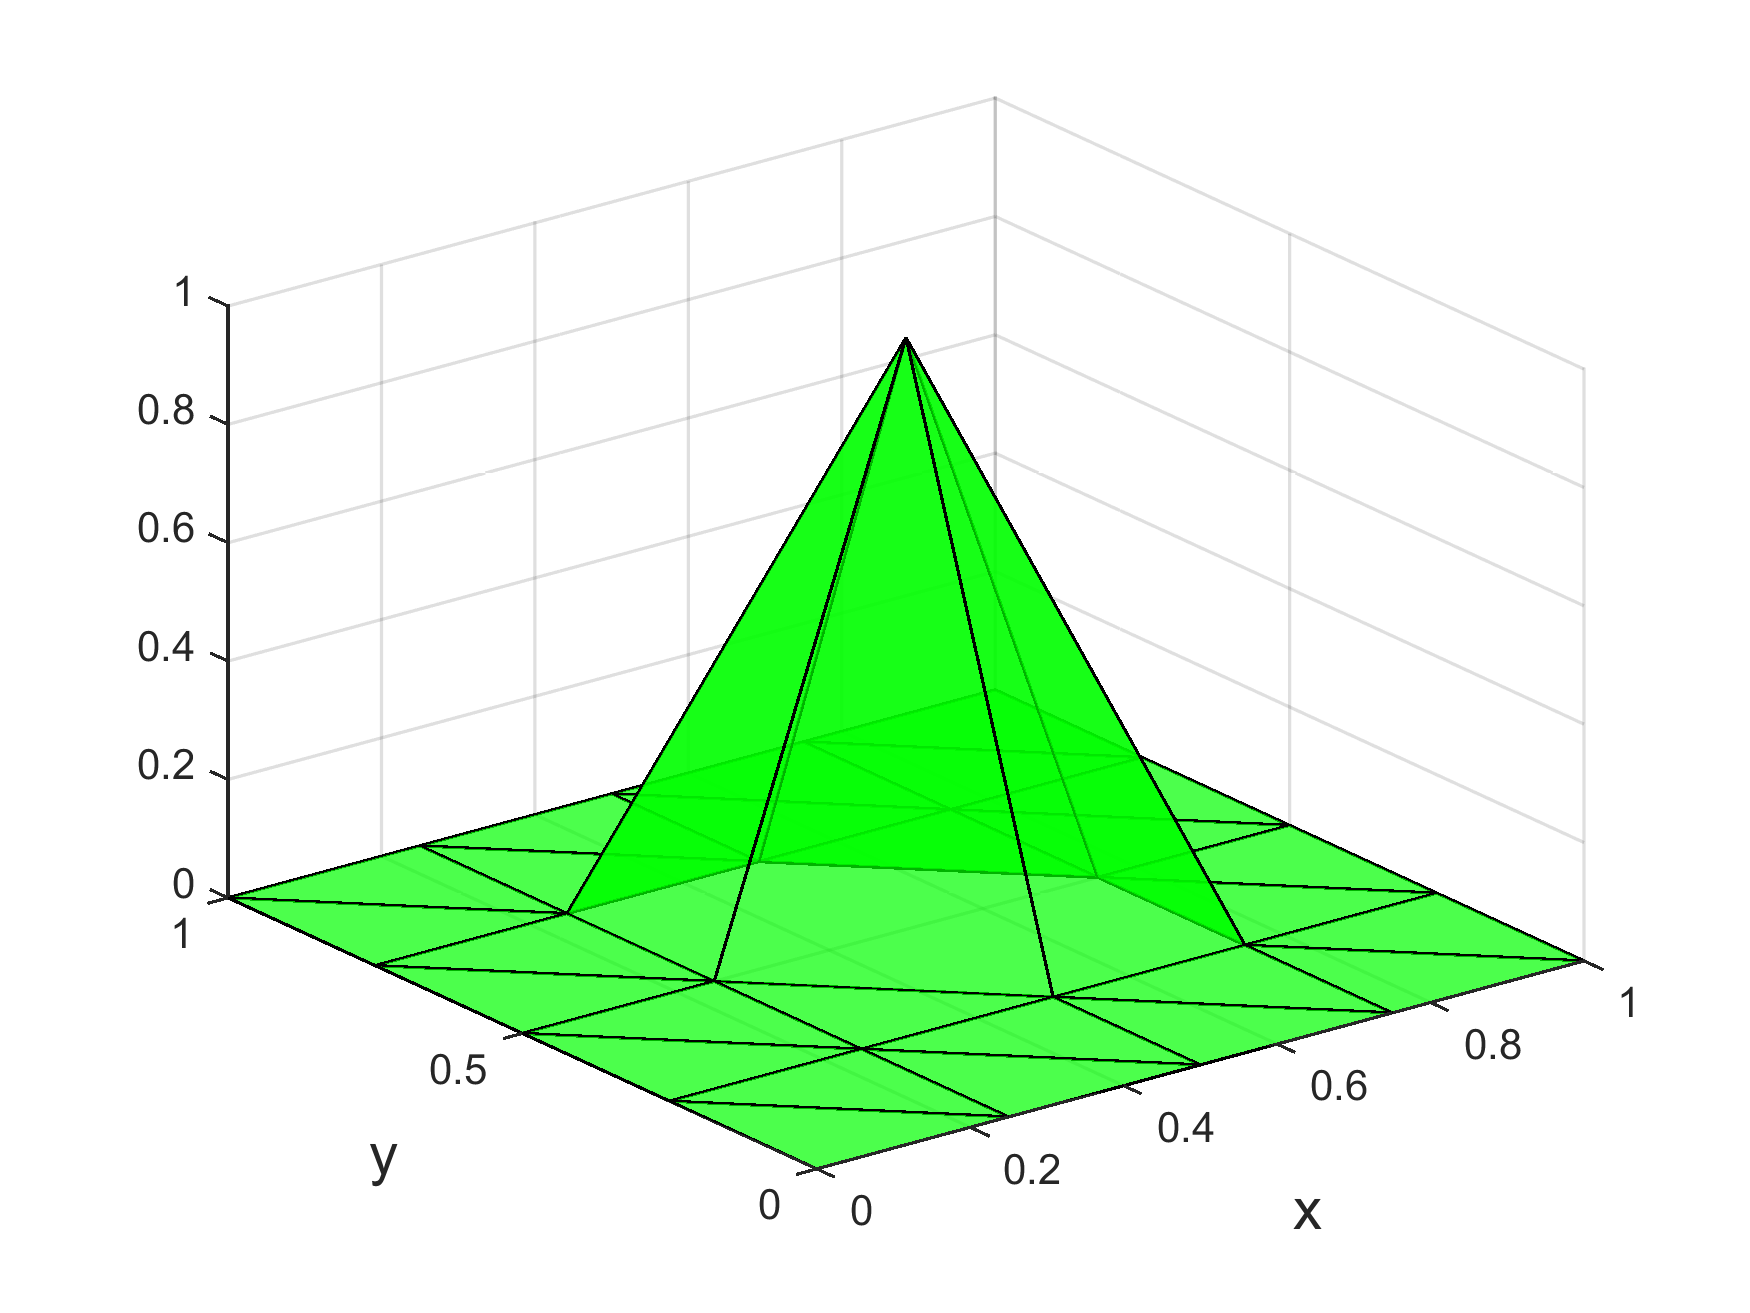
\includegraphics[width= .7\linewidth]{satorfv.png}}
		\label{fig:sator2d}
	\end{subfigure}
	\caption{\Aref{1dpelda}. példa $W_h$ altere a $[0,1]^2$ intervallumon: $u|_{T_k}$ folytonos, szakaszonként lineáris függvény (felső ábra), báziselemek a $\phi_{ij}(x_k,y_l) = \delta_{ik} \cdot \delta_{jl}$ sátorfüggvények (alsó ábra)}
	\label{fig:2dlinearis}
\end{figure}

\begin{example}\label{ddpelda}
	A fentiek általánosítása az $\Omega \in \R^d$ poliéder tartományon a $\mathbf{T_{d+1}^d}$ elem, ahol
	\begin{equation*}
		T_k: \text{nem elfajuló $d$-szimplex}, \quad u|_{T_k}: \text{lineáris függvény}, \quad (\forall T_k \in \mathcal{T}_h). 
	\end{equation*}
	A csomópontok a szimplexek csúcsai, ezekből $d+1$ darab van. A csúcsokban felvett értékek egyértelműen meghatározzák $u|_{T_k}$-t, $\forall  T_k \in \mathcal{T}_h$. Emellett $u$ a $d$-szimplex $d-1$ dimenziós lapjai mentén is értelmes, folytonos függvény, mivel két szomszédos $d$-szimplex  $d-1$ dimenziós közös lapján a csúcsbeli függvényértékek egyértelműen meghatározzák a közös lapon vett lineáris függvényt.  Az altér tehát
	\begin{equation*}
		W_h = \left\{ u \in C(\closure{\Omega}): u|_{T_k} \in P^1, \forall T_k \in \mathcal{T}_h  \right\}.
	\end{equation*}
\end{example}

További példák találhatók végeselemekre \acite{pdnm,stoyan3} jegyzetekben.






\chapter{Folytonos és diszkrét maximum-elvek elliptikus feladatra}\label{ch:Maxelvek}

Ebben a fejezetben először a folytonos maximum-elvet mutatjuk be \aref{ch:elmelet}. fejezetben definiált $L$ operátorra, és annak következményeit az operátor segítségével megfogalmazható Dirichlet-peremértékfeladatra. Ezután \aref{sec:classical_DMP}. részben rátérünk a feladat végeselemes approximációjára, és megfogalmazzuk a klasszikus diszkrét maximum-elvet, ami a szakaszonként lineáris közelítésre igazolható. Végül \ref{sec:general_DMP}. pontban ismertetjük az általánosított diszkrét maximum-elv ötletét  magasabbrendű közelítésekre.


 

\section{Folytonos maximum-elv}

Az itt bemutatott maximum-elvnél erősebb állítás is megfogalmazható az $L$ operátorra, azonban a végeselemes-módszerre ez a változat terjeszthető ki. A folytonos maximu-elvekkel bővebben foglalkozik pl. \cite{gilbarg}.

 
\Aref({L_op}) $L$ operátorra teljesül a következő tétel:

\begin{theorem} [Maximum-elv az $L$ operátorra]\label{cmp}
	Legyen $u \in C^2(\Omega) \cap C(\closure{\Omega})$, melyre $L u = f$ az $\Omega$ tartományon. Ha $f \leq 0$, akkor
	\begin{equation}
		\max_{\closure{\Omega}} u \leq \max \{0, \max_{\partial\Omega} u\},
	\end{equation}
	 és ha emellett $q \equiv 0$, akkor
	\begin{equation}
		\max_{\closure{\Omega}} u =  \max_{\partial\Omega} u .
	\end{equation}
\end{theorem}


\begin{proof} \cite{kar-kor}
	Legyen $v \in C^1(\closure{\Omega})$ és $v|_{\partial\Omega}=0$. Az $Lu$ kifejezést szorozzuk $v$-vel, és vegyük az integrálját $\Omega$-n. A Green-formula alkalmazásával az $L$ operátor divergencia-formáját kapjuk:
	\begin{equation}
	\label{div_form}
		\int_{\Omega} \left( p \grad u \cdot \grad v + q u v \right) = \int_{\Omega} f v 
	\end{equation}
	
	
	Legyen $M \coloneqq \max \{0, \max_{\partial\Omega} u\}$, és definiáljuk $v$-t a következőképp: $v \coloneqq \max \{u-M,0\}$. Ekkor $v$ definíció szerint szakaszonként $C^2$-beli, $v \geq 0$ és $v|_{\partial\Omega} = 0$. Mivel $f \leq 0$, \aref({div_form}) integrál jobb oldala:  $\int_{\Omega} f v  \leq 0$. 
	Jelölje $\Omega^{+} \coloneqq \{x \in \Omega : v(x) > 0\}$ halmazt. Ekkor az integrál $\Omega \setminus \Omega^{+}$-on 0, $\Omega^{+}$-on pedig $u = v + M$ adódik, így	
	\begin{equation*}
		0 \geq \int_{\Omega}  f v  = \int_{\partial\Omega} \left( p \grad u \cdot \grad v + q  u v \right) = \int_{\Omega^{+}} \left( p |\grad v|^2  + q  (v + M) v \right) \geq 0.
	\end{equation*}	
	Ebből $v$ konstans, és mivel $v|_{\partial\Omega} = 0$, így $v \equiv 0$, amiből $u \leq M$ adódik $\Omega$-n.
	
	Most tegyük fel, hogy $q = 0$. Mivel az integrálban ekkor a $q$-t tartalmazó tagok kiesnek, nem kell feltennünk, hogy $M \geq 0$. Legyen $M \coloneqq \max_{\partial\Omega} u$, $v$ pedig ugyanaz, mint az előző esetben. Ekkor a korábbiakhoz hasonlóan:	
	\begin{equation*}
		0 \geq \int_{\Omega} f v  = \int_{\partial\Omega}  p \grad u \cdot \grad v   = \int_{\Omega^{+}} p |\grad v|^2  \geq 0,
	\end{equation*}	
	amiből $v \equiv 0$ és $u \leq M$, így $\max_{\closure{\Omega}} u =  \max_{\partial\Omega} u$.
\end{proof}

\begin{corollary}[Maximum-elv Dirichlet-feladatra]\label{cmaxelv}
	Legyen $u \in C^2(\Omega) \bigcap C(\closure{\Omega})$ \aref({dirichlet_problem}) feladat megoldása. Ha $f \leq 0$ $\Omega$-n, akkor
	\begin{equation*}
		\max_{\closure{\Omega}} u \leq \max \{0, \max_{\partial\Omega} g\},
	\end{equation*}
	 és ha $q \equiv 0$, akkor
	\begin{equation*}
		\max_{\closure{\Omega}} u =  \max_{\partial\Omega} g .
	\end{equation*}
\end{corollary}

 Ebből azonnal következik a minimum-elv, ennek igazolásához elég $u$-t $-u$-val helyettesítenünk \eqref{dirichlet_problem}-ben.

\begin{corollary}[Minimum-elv Dirichlet-feladatra]\label{cminelv}
	Legyen $u \in C^2(\Omega) \bigcap C(\closure{\Omega})$ \aref({dirichlet_problem}) feladat megoldása. Ha $f \geq 0$ $\Omega$-n, akkor
	\begin{equation*}
		\min_{\closure{\Omega}} u \geq \min \{0, \min_{\partial\Omega} g\},
	\end{equation*}
	 és ha emellett $q \equiv 0$, akkor
	\begin{equation*}
		\min_{\closure{\Omega}} u =  \min_{\partial\Omega} g .
	\end{equation*}
\end{corollary}

A maximum- és minimum-elvekből közvetlenül adódnak a nempozitivitási és nemnegativitási tulajdonságok. 

\begin{corollary}[Nempozitivitási és nemnegativitási tulajdonság]
	Legyen $u \in C^2(\Omega) \bigcap C(\closure{\Omega})$ \aref({dirichlet_problem}) feladat megoldása. Ha $f \leq 0$ és $g \leq 0$, akkor $u \leq 0$, illetve ha $f \geq 0$ és $g \geq 0$, akkor $u \geq 0$ is teljesül.
\end{corollary}

\begin{remark}
	\Aref{cmp}. tétel és annak következményei kiterjeszthetők az $u \in H^1(\Omega)$ esetre, ha $u$ lényegében korlátos (azaz van olyan szám, ami majdnem mindenütt alsó/felső korlátja u-nak). Ekkor $\max{u}$ helyett a lényeges szuprémumot illetve infinumot kell vennünk \aref{cmp}. tételben, valamint \aref{cmaxelv}. és \ref{cminelv}. következményekben is $\closure{\Omega}$-n és $\partial\Omega$-n, továbbá \aref({dirichlet_problem}) feladatnál gyenge megoldást keresünk. 
\end{remark}

\section{Klasszikus diszkrét maximum-elv szakaszonként lineáris elemekre}\label{sec:classical_DMP}

Ebben a szakaszban bemutatjuk a klasszikus diszkrét maximum-elvet. A tétel a szakaszonként lineáris függvényekkel való végeselemes approximációnál a tartomány felosztásának szögeire tett feltétel mellett teljesül. Azonban \aref{sec:general_DMP}. fejezetben látni fogjuk, hogy a magasabb fokú végeselemes közelítések (hp-FEM) esetén már egy dimenziós tartományon is van ellenpélda. 

% [Klasszikus diszkrét maximum-elv inhomogén Dirichlet-feladatra]
\begin{definition}\label{cDMP}
	\Aref({inhom_vetegy}) inhomogén Dirichlet-feladat kielégíti a klasszikus diszkrét maximum-elvet, ha  $\forall f \leq 0$ esetén az $u_h$ megoldásra teljesül:
	\begin{equation}\label{eq:cDMP_alt}
		\max_{\closure{\Omega}} u_h \leq \max \{0, \max_{\partial\Omega} g_h\},
	\end{equation}
	emellett, ha $q \equiv 0$, 
	% és a $W_h$ bázisfüggvényeire teljesül, hogy $\sum_{j = 1}^{n+m}\varphi_{j} \equiv const $ az $\closure{\Omega}$-n, 
	akkor
	\begin{equation}\label{eq:cDMP_alt_0q}
		\max_{\closure{\Omega}} u_h =  \max_{\partial\Omega} g_h.
	\end{equation}
	A fenti kifejezésekben $g_h$ a g peremfeltétel $W_h$-beli polinomiális interpolációja.
\end{definition}

A következőkben elégséges feltételt mutatunk a klasszikus diszkrét maximum-elv teljesülésére a szakaszonként lineáris végeselemek alkalmazás esetén.

\subsection{Mátrix maximum-elv}

Először fogalmazzuk meg az inhomogén Dirichlet-feladathoz tartozó lineáris egyenletrendszer szintjén a maximum-elvet. A következő szakaszban látni fogjuk, hogy lineáris végeselemek alkalmazásakor a mátrixokra megfogalmazott maximum-elv teljesülése elégséges feltételt szolgáltat \aref{cDMP}. klasszikus maximum-elv teljesülésére.

\begin{definition}\label{irrdiagdomdef}
	Az  $n$ dimenziós négyzetes $\mx{M} = (m_{ij})_{i,j=1}^n$ mátrixot irreducibilisen diagonálisan dominánsnak nevezzük, ha kielégíti a következő feltételeket:
	\begin{enumerate}[label=(\alph*)]
		\item $\mx{M}$ irreducibilis, azaz $\forall i \neq j$ esetén létezik $\mx{M}$ elemeinek egy nemnulla $ \{m_{i,i_1}, m_{i_1,i_2}, \ldots, m_{i_s,j} \}$ sorozata, ahol $i, i_1, \ldots, i_s, j$ különböző indexek,\label{irredfelt}
		\item $\mx{M}$ diagonálisan domináns, azaz  \label{diagdomfelt}
			\begin{equation*}
				|m_{i,i}| \geq \sum_{\substack{j = 1 \\ j \neq i}}^n |m_{i,j}|, \quad i = 1, \ldots, n,
			\end{equation*}
		\item $\mx{M}$-nek legalább az egyik sora szigorúan diagonálisan domináns, azaz $\exists i_0 \in \{1, \ldots, n\}$, melyre \label{szigdiagdomfelt}
			\begin{equation*}
				|m_{i_0,i_0}|  > \sum_{\substack{j = 1 \\ j \neq i_0}}^n |m_{i_0,j}|
			\end{equation*}
	\end{enumerate}
\end{definition}

\begin{theorem}\label{poz_inverz_tetel}
	Ha az  $n$ dimenziós négyzetes $\mx{M} = (m_{ij})_{i,j=1}^n$ mátrix irreducibilisen diagonálisan domináns,  $m_{ij} \leq 0$, ha $i \neq j$ és $m_{ii} > 0$ minden $i = 1, \leq, n$ esetén, akkor $\mx{M}^{-1} > 0$.
\end{theorem}

A tétel bizonyítása megtalálható \cite{varga} 85. oldalán. 
 	
\begin{theorem}[Mátrix maximum-elv]\label{mx_max_tetel}
	Tekintsük \aref({inhom_mx_def}) pontban definiált $\mx{\widehat{A}_h} = (a_{ij})_{i,j=1}^{n+m} \in \R^{(n+m) \times (n+m)}$ mátrixot és $\vr{\widehat{c}_h} = (c_1, \ldots, c_{n+m})^T \in \R^{n+m}$ vektort. Tegyük fel, hogy $\mx{\widehat{A}_h}$-ra teljesülnek a következő feltételek:
	\begin{enumerate}[label=(\roman*)]
		\item $a_{ii} > 0, \quad i = 1, \ldots, n$,\label{A_diag_poz}
		\item $a_{ij} \leq 0, \quad i = 1, \ldots, n,\, j = 1, \ldots, n+m,\, i \neq j$,
		\item $\displaystyle \sum_{j = 1}^{n+m} a_{ij} \geq 0,  \quad i = 1, \ldots, n$, \label{nemneg_sorosszeg}
		\item $\mx{A_h}$ ireducibilisan diagonálisan domináns.\label{A_irreddd}
	\end{enumerate}
	Ekkor ha a $\vr{\widehat{c}_h}$ olyan, hogy $(\mx{\widehat{A}_h} \vr{\widehat{c}_h})_i \leq 0 $, minden $i = 1, \ldots, n$, akkor
	\begin{equation}\label{eq:cDMP_mx}
		\max_{ 1 \leq i \leq n+m} c_i \leq \max \left\{0, \max_{n+1 \leq i \leq n+m} c_i \right\},
	\end{equation}
	és ha ezen felül 
	\begin{equation}\label{eq:nullsorosszeg_felt}
		\sum_{j = 1}^{n+m} a_{ij} = 0,  \quad i = 1, \ldots, n
	\end{equation}
	is teljesül, akkor
	\begin{equation}\label{eq:cDMP_mx_0q}
		\max_{1 \leq i \leq n+m} c_i =  \max_{n+1 \leq i \leq n+m} c_i .
	\end{equation}
\end{theorem}

\begin{proof} \cite{kar-kor}
	Tekintsük a $\vr{\widehat{c}_h}$ vektor kövektező felbontását: $\vr{\widehat{c}_h} = (\vr{c_h} ,\vr{g_h})^T $, ahol $\vr{c_h} = (c_1, \ldots, c_{n})^T$ és $\vr{g_h} = (c_{n+1}, \ldots, c_{n+m})^T$. Tegyük fel, hogy $\mx{A_h}\vr{c_h} + \mx{\tilde{A}_h} \vr{g_h} \leq 0 \in \R^n$. Ekkor azt kapjuk, hogy $\vr{c_h} \leq -\mx{A_h}^{-1} \mx{\tilde{A}_h} \vr{g_h}$, ahol az $ - \mx{A_h}^{-1} \mx{\tilde{A}_h}$ mátrix nemnegatív, hiszen a tétel feltevései és \aref{poz_inverz_tetel}. tétel miatt $\mx{A_h}^{-1} > 0$ és $\mx{\tilde{A}_h} \leq 0$. 
	
	Legyen  $\vr{1} = (1, \ldots, 1)^T \in \R^n$ és  $ \vr{\tilde{1}} = (1, \ldots, 1)^T \in \R^m$. Ekkor \ref{nemneg_sorosszeg} miatt $\mx{A_h}\vr{1} + \mx{\tilde{A}_h}\vr{\tilde{1}} \geq 0 \in \R^n$, azaz $\vr{1} \geq - \mx{A_h}^{-1} \mx{\tilde{A}_h} \vr{\tilde{1}}$.
	
	Az előzőekből adódóan   $\vr{c_h}$ vektor felülről becsülhető:
	\begin{align*}	
		\vr{c_h} &\leq -\mx{A_h}^{-1} \mx{\tilde{A}_h} \vr{g_h} \leq \max \left\{0, \max_{n+1 \leq i \leq n+m} c_i \right\}  (- \mx{A_h}^{-1} \mx{\tilde{A}_h} \vr{\tilde{1}}) \leq \\
		&\leq \max \left\{0, \max_{n+1 \leq i \leq n+m} c_i \right\} \vr{1},
	\end{align*}
	amiből \eqref{eq:cDMP_mx} következik.
	
	Ha \aref({eq:nullsorosszeg_felt}) feltétel teljesül, azt felhasználva $\mx{A_h}\vr{1} + \mx{\tilde{A}_h}\vr{\tilde{1}} = 0 \in \R^n$, tehát $\vr{1} = - \mx{A_h}^{-1} \mx{\tilde{A}_h} \vr{\tilde{1}}$ adódik. A $\vr{c_h}$ vektor felső becslésénél az egyenlőség miatt elhagyhatjuk a nemnegativitási feltételt:
	\begin{equation*}
		\vr{c_h} \leq -\mx{A_h}^{-1} \mx{\tilde{A}_h} \vr{g_h} \leq \left( \max_{n+1 \leq i \leq n+m} c_i \right) (- \mx{A_h}^{-1} \mx{\tilde{A}_h} \vr{\tilde{1}}) = \left( \max_{n+1 \leq i \leq n+m} c_i \right)\vr{1},
	\end{equation*}
	és ebből következik  \eqref{eq:cDMP_mx_0q}.	
\end{proof}

\begin{remark}\label{rem:qqphi_felt}
	Abban az esetben, ha $q \equiv 0$, akkor  $a(1,\varphi_i) = 0$ teljesül minden $i = 1, \ldots, n$ esetén. Ha ezen felül a bázisfüggvényekre $\sum_{j = 1}^{n+m}\varphi_{j} \equiv 1 $ teljesül $\closure{\Omega}$-n, akkor minden $i = 1, \ldots, n$ esetén teljesül \aref{mx_max_tetel}. tételbeli \eqref{eq:nullsorosszeg_felt} feltétel, ugyanis:
	\begin{equation*}
		\sum_{j = 1}^{n+m} a(\varphi_j,\varphi_i) = a\left( \left( \sum_{j = 1}^{n+m}\varphi_{j}\right), \varphi_i \right) = a(1,\varphi_i) = 0.
	\end{equation*}
\end{remark}	

\begin{remark}
	\Aref{mx_max_tetel}. tételben \aref({eq:nullsorosszeg_felt}) állítás a $g \leq 0$ esetben magába foglalja a nempozitivitási tulajdonságot, ugyanis ekkor $c_i \leq 0, i = n+1, \ldots ,n+m$, amiből az állítás miatt:
	\begin{equation*}
		\max_{1 \leq i \leq n+m} c_i \leq 0.
	\end{equation*}
\end{remark}	
	
\begin{remark}
	\Aref{mx_max_tetel}. tételből adódóan homogén Dirichlet-feladat esetén szintén teljesül a nempozitivitási feltétel. Ebben az esetben  $c_i = 0, i = n+1, \ldots ,n+m$, ezért \aref({inhom_ler})-beli $\mx{A_h}\vr{c_h} + \mx{\tilde{A}_h} \vr{g_h} = \vr{b_h}$ lineáris egyenletrendszer \aref({lin_rsz})-ben adott $\mx{A_h}\vr{c_h} = \vr{b_h}$ alakra redukálódik, ahol $\mx{A_h}$ \ref{A_irreddd} miatt irreducibilisen diagonálisan domináns. Az $(\mx{A_h}\vr{c_h})_i \leq 0, i = 1, \ldots, n$ feltételből ekkor
	\begin{equation*}
		\max_{1 \leq i \leq n} c_i \leq 0
	\end{equation*}
	adódik, ami analóg a tételbeli \eqref{eq:nullsorosszeg_felt} állítással.
\end{remark}	

\begin{remark}
	\Aref{mx_max_tetel}. tétel \eqref{eq:cDMP_mx} és  \eqref{eq:cDMP_mx_0q} állításai analóg diszkrét megfogalmazásai  \aref{cDMP}. klasszikus maximum-elv \eqref{eq:cDMP_alt} és \eqref{eq:cDMP_alt_0q} állításainak. 
\end{remark}	





\subsection{A lineáris végeslemekre tett elégséges kikötések}

Ebben a részben először megmutatjuk, hogy a \ref{ddpelda}. példában bemutatott $\mathbf{T_{d+1}^d}$ végeselemek alkalmazásakor a mátrix maximum-elv teljesülése elégséges feltétel a klasszikus maximum-elvre, ezután pedig elégséges feltételt mutatunk a mátrix maximum-elv, és így a klasszikus maximum-elv teljesülésére. Az itt bemutatott eredményekkel  pl. \cite{ciarlet-raviart} foglalkozik.

Lineáris végeselemes közelítés esén $\forall T_k \in \mathcal{T}_h$ elemre $u_h|_{T_k}$ lineáris, ezért $u_h|_{T_k}$ csak a $T_k$ elem csúcsaiban veheti fel maximumát. Így elegendő \aref{cDMP}. klasszikus maximum-elvet az $u_h$ függvény rácscsomópontokban felvett értékeire igazolnunk.

Tekintsük az $\Omega \in \R^d$ poliéder tartomány egy $\mathcal{T}_h = \{ T_1, \ldots, T_M \}$  triangulációját, melynek elemei nem elfajuló $d$-szimplexek. Legyenek  $B_i, i=1, \ldots, n+m$ a csúcsok $\mathcal{T}_h$-ban, ahol $B_i$ az $i=1, \ldots, n$ indexekre a belső csúcsokat, $i = n+1, \ldots, n+m$ indexekre pedig a $\partial\Omega$-n lévő csúcsokat jelöli. Legyen $W_h$  a szakaszonként lineáris függvények tere, ahol  bázist alkotnak a $\varphi_i(B_j) = \delta(i,j), \,  i,j=1, \ldots, n+m$  feltétellel definiált függvények. Ekkor az $u_h \in W_h$ közelítésnek a peremen felvett értékei: $c_{n+j} = g_j = g(B_{n+j})$, ha $ j = 1, \ldots, m$. Keressük az $u_h$ megoldásnak a  belső csúcsokhoz tartozó $c_1, \ldots, c_n$  értékeit.

Az $f \leq 0$ feltételből lineáris esetben következik $(\mx{\widehat{A}_h} \vr{\widehat{c}_h})_i \leq 0 $, minden $i = 1, \ldots, n$ esetén, mert $ \varphi_i \geq 0, \, (i = 1, \ldots, n)$, és így $l(\varphi_i) \leq 0 \, (i = 1, \ldots, n)$ teljesül. \Aref{sec:general_DMP} fejezetben látni fogjuk, hogy  magasabbrendű végeselemes közelítések esetén $f$ nempozitivitásából nem következik a jobboldal nempozitivitása, ezért ezekben az esetekben más feltételhez kell kötnünk a maximum-elv teljesülését.

Lineáris esetben a  bázisra a $\sum_{j = 1}^{n+m}\varphi_{j} \equiv 1 $   teljesül, így \aref{rem:qqphi_felt}. megjegyzés miatt $q \equiv 0$ feltételből következik  \aref{mx_max_tetel}. tételbeli \eqref{eq:nullsorosszeg_felt} feltétel, azaz ekkor a merevségi mátrix minden sorösszege $0$.

A fentiek alapján lineáris végeselemes approximációnál, ha az $\mx{\widehat{A}_h}$ merevségi mátrixra \aref{mx_max_tetel}. tételben adott  \ref{A_diag_poz}-\ref{A_irreddd} feltételek teljesülnek, akkor \aref{cDMP}. klasszikus maximum-elv is teljesül az inhomogén Dirichlet-feladatra. Ezen feltételek biztosítására szintén van elégséges feltétel. Ekkor a trianguláció megfelelő finomsága mellett a rácsra tett szögfeltétellel biztosíthatók az  $\mx{\widehat{A}_h}$ merevségi mátrix megfelelő tulajdonságai.

Tekintsünk egy $T_k \in \mathcal{T}_h$ $d$-szimplexet. Jelölje $\hat{B_r}, \, r = 1, \ldots, d+1$ a csúcsait, és legyenek  $\hat{\varphi_r}, \, r = 1, \ldots, d+1$ a megfelelő bázisfüggvények megszorításai $T_k$-ra. Ekkor tehát $\hat{\varphi_r}(\hat{B_s}) = \delta(r,s), $ minden $ r,s = 1, \ldots, d+1$ esetén. A bevezetett jelölések segítségével definiálhatjuk a $T_k$ elem egy jellemző paraméterét:
\begin{equation*}
	\sigma(T_k) \coloneqq  \max_{\substack{1 \leq r,s \leq d+1 \\ r \neq s}}\{  \cos (\grad \hat{\varphi_r}, \grad \hat{\varphi_s}) \}.	
\end{equation*}
Ekkor a $\mathcal{T}_h $ trianguláció jellemezhető  a következő paraméterekkel: 
\begin{align*}
	 h &=  \max_{T_k \in \mathcal{T}_h} diam(T_k),	\\	
	 \sigma(h) &\coloneqq  \max_{T_k \in \mathcal{T}_h} \sigma(T_k),		
\end{align*}
ahol $h$ megegyezik a korábban \ref{def:finomság}. pontban definiált finomsággal. 

\begin{statement}\label{cDMP_telj}
	Tekintsük a $\mathcal{T}_h$ triangulációk egy sorozatát, ahol $h \rightarrow 0$. Ekkor \aref{cDMP}. klasszikus maximum-elv teljesül, ha 
	\begin{align}
		&\exists \sigma_0 > 0 \text{ úgy, hogy } \sigma(h) \leq -\sigma_0 < 0 \, (\forall h), \label{szogfelt} \\
		& h  \text{ elegendően kicsi} \label{hfelt}
	\end{align}
\end{statement}

% \{\interior{T_k}: T_k \in \mathcal{T}_h, valamint T_k csúcsai közt szerepel B_i és B_j\}

\begin{proof}
	Az előzőek alapján  \aref{cDMP}. klasszikus maximum-elv teljesüléséhez elég belátni, hogy az $\mx{\widehat{A}_h} = (a_{ij})_{i,j=1}^{n+m}$ merevségi mátrixra igazak \aref{mx_max_tetel}. tételben adott  \ref{A_diag_poz}-\ref{A_irreddd} feltételek. 
	\begin{enumerate}[label=(\roman*)]
		\item Az $a(.,.)$ bilineáris forma koercivitása miatt $a_{ii} = a(\varphi_i,\varphi_i) > 0, \forall i = 1, \ldots, n$.
		\item Tegyük fel, hogy \eqref{szogfelt} teljesül, és $i \neq j$. Definiáljuk $\Omega_{ij} \coloneqq   \supp \varphi_i \cup \supp \varphi_j$ tartományt. Ekkor az $a(\varphi_i,\varphi_i)$ bilineáris forma az $\Omega \setminus \Omega_{ij}$ tartományon $0$, ezért:
			\begin{align*}
				a_{ij} &= a(\varphi_j,\varphi_i) =  \int_{\Omega_{ij}} \left( p \grad \varphi_j \cdot \grad \varphi_i  + q \varphi_j \varphi_i \right) = \\
				&= \sum_{T_k \in \Omega_{ij}} \int_{T_k} \left( p \grad \varphi_j \cdot \grad \varphi_i  + q \varphi_j \varphi_i \right).
			\end{align*}
			
			Rögzítsünk egy $T_k \in \Omega_{ij}$ elemet. A $p$ alulról korlátos, jelölje az alsó korlátját $m$. Ekkor
			\begin{align*}
				 &\int_{T_k} \left( p \grad \varphi_j \cdot \grad \varphi_i  + q \varphi_j \varphi_i \right) \leq \\ 
				 \leq  &m \sigma(h) \int_{T_k} \underbrace{|\grad \varphi_j|}_{\geq \frac{1}{h}} \underbrace{|\grad \varphi_i|}_{\geq \frac{1}{h}}   + \|q\|_{L^{\infty}(\Omega)} \int_{T_k} \underbrace{\varphi_j}_{\leq 1} \underbrace{\varphi_i}_{\leq 1} \leq \\
				 \leq &\left(-\frac{\sigma_0}{h^2} m + \|q\|_{L^{\infty}(\Omega)}\right)  \lambda(T_k) \leq 0,
			\end{align*}
			 ha $h$ elég kicsi, azaz \eqref{hfelt}. A $\lambda(T_k)$ a $T_k$ $d$-szimplex Lebesgue-mértékét jelöli. Vegyük észre, hogy ha $h$ elég kicsi, akkor $<$ reláció is teljesül, azaz $a_{ij} < 0$, ha $i = 1, \ldots, n, \, j = 1, \ldots, n+m, \, i \neq j$. 
			 \label{szigpozbiz}
		\item A bázisfüggvényekre $\sum_{j = 1}^{n+m}\varphi_{j} \equiv 1 $ teljesül, emiatt:
			\begin{align*}
				\sum_{j = 1}^{n+m} a_{ij} &= \sum_{j = 1}^{n+m} a(\varphi_j,\varphi_i) = \sum_{j = 1}^{n+m} \int_{\Omega} \left( p \grad \varphi_j \cdot \grad \varphi_i  + q \varphi_j \varphi_i \right) 	\\						
				&=  \int_{\Omega}  p \grad \varphi_i \cdot \grad \underbrace{\left(\sum_{j = 1}^{n+m} \varphi_j \right)}_{\equiv 1}    + \int_{\Omega} q  \varphi_i \underbrace{\left(\sum_{j = 1}^{n+m} \varphi_j \right)}_{\equiv 1} 
				= \int_{\Omega} \underbrace{q}_{\geq 0} \underbrace{\varphi_i}_{\geq 0}	\geq 0.
			\end{align*}
		\item  $\mx{A_h}$ irreducibilitása abból adódik, hogy tetszőleges $B_i, B_j$ csúcsokhoz, ahol $i \neq j$, van különböző csúcsoknak olyan $\{ B_i = B_{i_0}, B_{i_1}, \ldots, B_{i_s}= B_j \}$ sorozata, amelynek bármely két egymást követő $B_{i_r}, B_{i_{r+1}}, (0 \leq r \leq s-1)$ elemeihez tartozó $\varphi_{i_r}, \varphi_{i_{r+1}} $  bázisfüggvényekre $\supp \varphi_{i_r} \cap \supp \varphi_{i_{r+1}} \neq \emptyset$ teljesül. \Aref{szigpozbiz} pontban beláttuk, hogy megfelelően kicsi $h$ esetén $a_{ij} < 0$, ha $i \neq j$, ezért van olyan $h$, amivel $a_{i_r,i_{r+1}} < 0, (0 \leq r \leq s-1)$ teljesül. Ekkor tehát igaz \aref{irrdiagdomdef}-beli \ref{irredfelt} feltétel.

			\Aref{irrdiagdomdef}-beli \ref{diagdomfelt} és \ref{szigdiagdomfelt} igazolásához tekintsük \ref{nemneg_sorosszeg} feltételt. Tegyük fel, hogy $h$ elegendően kicsi, és így $a_{ij} < 0$, ha $i = 1, \ldots, n, \, j = 1, \ldots, n+m, \, i \neq j$ . Ekkor tetszőleges $1 \leq i \leq n$ esetén
			\begin{equation*}
				\sum_{j = 1}^{n+m} a_{ij} = \underbrace{a_{i,i}}_{\substack {>0 \\ (i)-ből}} + \sum_{\substack {j = 1 \\ i \neq j}}^{n} \underbrace{a_{ij}}_{<0} + \sum_{j = n+1}^{n+m} \underbrace{a_{ij}}_{<0} = |a_{i,i}| - \sum_{\substack {j = 1 \\ i \neq j}}^{n} |a_{ij}| - \sum_{j = n+1}^{n+m} |a_{ij}| \geq 0.
			\end{equation*}
			Ezt átalakítva
			\begin{equation*}
				|a_{i,i}| - \sum_{\substack {j = 1 \\ i \neq j}}^{n} |a_{ij}| \geq \sum_{j = n+1}^{n+m} \underbrace{|a_{ij}|}_{> 0} > 0,
			\end{equation*}
			azaz 
			\begin{equation*}
				|a_{i,i}| > \sum_{\substack {j = 1 \\ i \neq j}}^{n} |a_{ij}|.
			\end{equation*}
			Tehát ekkor \aref{irrdiagdomdef}-beli   \ref{diagdomfelt} és  \ref{szigdiagdomfelt} feltétel is teljesül, ha $h$ elegendően kicsi.
	\end{enumerate}
\end{proof}

\begin{remark}\label{2dszogfelt}
	2D-ben \eqref{szogfelt} pontosan akkor teljesül, ha $\exists \epsilon > 0$ úgy, hogy $\forall h$-ra $\forall T_k \in \mathcal{T}_h$ háromszög minden $\alpha$ belső szögére $\alpha \leq \pi / 2 - \epsilon$ teljesül, azaz a végeselemes rács minden szöge egyenletesen hegyesszög. Abban az esetben, ha $q \equiv 0$, akkor $\epsilon = 0$ is megengedett, azaz a rácsban ekkor derékszögek is lehetnek.
\end{remark}		



\section{Általánosított diszkrét maximum-elv magasabbrendű elemekre}\label{sec:general_DMP}

Ebben a szakaszban az 1 dimenziós Poisson-egyenlet végelselemes approximációját vizsgáljuk.  Először egy ellenpéldán keresztül igazoljuk, hogy a klasszikus diszkrét maximum-elv nem terjeszthető ki a magasabbrendű végeselemes közelítésekre (hp-FEM). Ennek az az oka, hogy a jobb oldali $f$ függvény nempozitivitásából nem feltétlenül következik $l(.)$ korlátos lineáris funkcionál nempozitivitása. A probléma kiküszöbölésésre kimondjuk az általánosított diszkrét maximum-elvet, ami a nempozitivitást az $f$ függvény helyett annak $V_h$ térbeli $L^2$-vetületére feltételezi. Végül megmutatjuk, hogy az általánosított diszkrét maximum-elv  bizonyos feltevések mellett igazolható magasabbrendű közelítésekre is. A szakaszban bemutatott eredmények \cite{sol-vej}-ből származnak. 

Tekintsük az $\Omega = (a,b)\in \R$ intervallumon a $-u'' = f$ Poisson-egyenletet homogén Dirichlet-peremmel, azaz $u(a) = u(b) = 0$. Ez a korábban definiált \eqref{dirichlet_problem} feladatnak a $p \equiv 1 $ és $q \equiv 0$ esete. A gyenge feladat ekkor: adott $f \in L^2(\Omega)$ mellett keressük azt az $u \in H_0^1(\Omega)$ függvényt, amelyre
\begin{equation} \label{1dgyenge}
	\int_{a}^{b} u'(x)v'(x) \dd x =  \int_{a}^{b} f(x)v(x) \dd x, \quad (\forall v \in H_0^1(\Omega)).
\end{equation}

Tegyük fel, hogy $f \in L^2(\Omega)$, és osszuk fel  $\closure{\Omega}$-t $M$  darab szakaszra: $a = x_0 < x_1 < \ldots < x_M = b$. Ekkor a $\mathcal{T}_h$ trianguláció elemei a $T_k = [x_{k-1},x_k]$ intervallumok. A $V_h \subset H_0^1(\Omega)$ altér legyen most a
szakaszonként polinom függvények tere:
\begin{equation*}
	V_h = \left\{ u \in C(\closure{\Omega}): u|_{T_k} \in P^{p_k}, \forall T_k \in \mathcal{T}_h  \text{ és } u(a) = u(b) = 0 \right\}.
\end{equation*}

A végeselemes feladat tehát: keressük azt az $u_h \in V_h$ függvényt, amire teljesül a következő:
\begin{equation}\label{diszkret1d}
	\int_{a}^{b} u_h'(x)v_h'(x) \dd x =  \int_{a}^{b} f(x)v_h(x) \dd x, \quad (\forall v_h \in V_h).
\end{equation}

\begin{definition}
	\Aref({diszkret1d}) diszkrét feladatban jelölje az $f \in L^2(\Omega)$  függvény $V_h$ altérre vett $L^2$-vetületét $f_h \in V_h$ , ha $f_h$-ra teljesül:
	\begin{equation}\label{f_hdef}
		\int_a^b (f_h(x) - f(x)) v_h(x) \dd x = 0 \quad (\forall v_h \in V_h).
	\end{equation}
\end{definition}
\begin{remark}
	\Aref({f_hdef}) egyenletet átalakítva
	\begin{equation}
		\int_a^b f_h(x) v_h(x) \dd x  =  \int_a^b f(x) v_h(x) \dd x  = 0 \quad (\forall v_h \in V_h), 
	\end{equation}
	tehát a diszkrét feladat megoldásánál a tehervektort az $f$ és az $f_h$ függvényből számolva ugyanazt kapjuk.
\end{remark}

\subsection{Ellenpélda a klasszikus diszkrét maximum-elv kiterjesztésére magasabbrendű közelítésre}

Megmutatható, hogy \aref{cDMP}. klasszikus diszkrét maximum-elv már a harmadrendű végeselemek esetére sem terjeszthető ki, tehát amikor $u|_{T_k} \in P^{p}$, ahol $p = 3 \, (\forall T_k \in \mathcal{T}_h) $. Ennek bizonyításához tekintsük az Lobatto-polinomokat a $[-1, 1]$ intervallumon:
\begin{equation}\label{lobatto}
	l_k(x)= \int_{-1}^x L_{k-1}(\xi) \dd \xi, \quad 2 \leq k,
\end{equation}
ahol $L_{k-1}$ a normált $k-1$ fokú Legendre-poninomot jelöli. Ekkor $l_2, l_3, \ldots$ függvények $\pm 1$-ben $0$ értéket vesznek fel, és a $H_0^1$-beli skaláris szorzásra nézve ortonormáltak:
\begin{equation}\label{eq:legendre_on}
	\langle l_i, l_j \rangle_{H^1_0(\Omega)} = \int_{-1}^x l_i'(x)  l_j'(x) \dd x = \delta_{ij}, \quad 2 \leq i,j.
\end{equation}


\begin{example}\label{bukaspelda}
	Az $\Omega = (-1,1)$ intervallumon tekintsük a $\mathcal{T}_h = \{T_1\} = \{[-1,1]\}$ triangulációt. Harmadfokú közelítés esetén a $V_h$ altér bázisát alkotják az $l_2, l_3$ függvények, és a közelítő megoldás felírható $u_h = y_1 l_2(x) + y_2 l_3(x)$ alakban. Ekkor \eqref{eq:legendre_on} miatt a merevségi mátrix a $2 \times 2$ dimenziós egységmátrix, és az ismeretlen $y_1, y_2$ együtthatók felírhatók a következőképp:
	\begin{equation}
		y_i = \int_{-1}^1 \sum_{j=1}^2 y_i l_{j+1}'(x) l_{i+1}'(x) \dd x = \int_{-1}^1 f(x) l_{i+1}(x) \dd x, \quad i = 1,2.
	\end{equation}
	Legyen $f$ a következő: 
	\begin{equation}\label{eq:bukaspelda_rhs}
		f = 200 e^{-10(x+1)}.
	\end{equation}
	Ekkor az együtthatókra azt kapjuk, hogy:
	\begin{align*}
		y_1 & = -\sqrt{6}\frac{(9 + 11 e^{-20})}{10}, & y_2 & = \sqrt{10}\frac{(73 - 133 e^{-20})}{100}. 
	\end{align*}
	Tehát $u$-ra a végeselemes közelítés:
	\begin{equation}
		u_h(x) = \frac{1}{40} (1-x^2) (54 + 66 e^{-20} - (73 - 133 e^{-20})x). 
	\end{equation}
	\Aref{fig:solvejbukas} bal oldali ábrán látható, hogy $u_h$ negatív értékeket is felvesz az $\Omega$-n, tehát \aref{cDMP}. klasszikus diszkrét maximum-elv ekkor nem teljesül.
	
	 Ahhoz, hogy megértsük, miért nem igaz a feladatra \aref{cDMP}., vizsgáljuk meg az $f_h$ vetületet. Írjuk fel $f_h$-t az $l_2,l_3$ bázisfüggvények segítségével. Ezt \eqref{f_hdef}-be helyettesítve egy lineáris egyenletrendszert kapunk, amit megoldva:
	\begin{equation}
		f_h(x) = \frac{3}{80} (1-x^2) (110 e^{-20} + 90 + ( 931 e^{-20} - 511)x). 
	\end{equation}
	Ekkor, mint ahogy  \aref{fig:solvejbukas} jobb oldali ábrán megfigyelhető, $f_h$ negatív értékeket is felvesz az $\Omega$-n. Ez azt jelenti, hogy nem teljesül \aref({diszkret1d}) diszkrét feladatban a jobb oldal nemnegativitása vagyis nem teljesül a mátrix maximum-elv egyik feltétele.		
\end{example}

\begin{figure}[h]
	\centerline{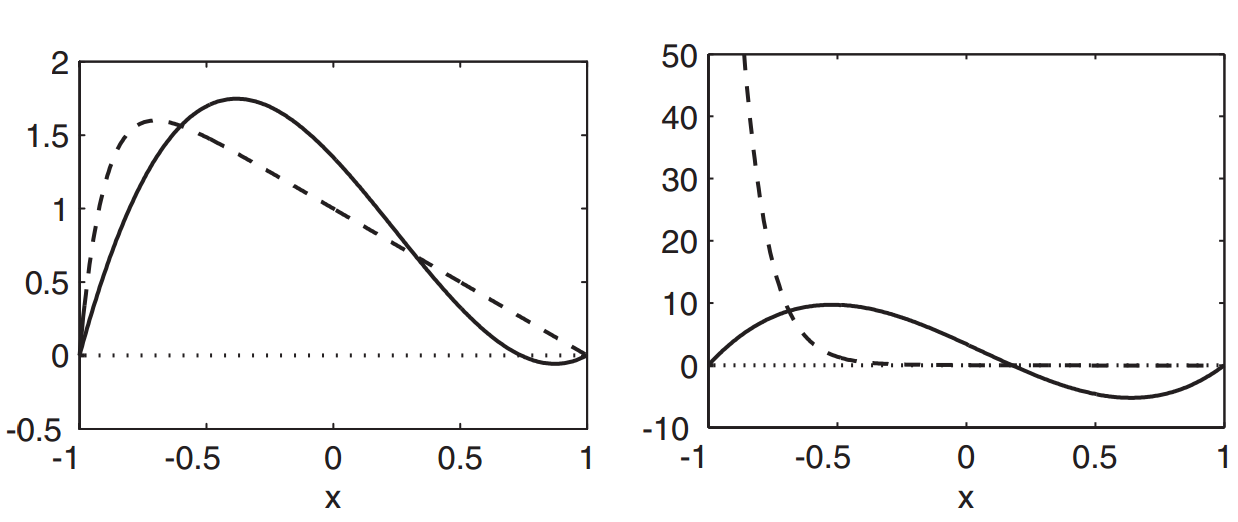
\includegraphics[width=.8\linewidth]{solvejbukas.png}}
	\caption{Bal oldalon: \aref{bukaspelda}. példa harmadfokú közelítése (folytonos vonallal), és a pontos megoldás (szaggatott vonallal). Jobb oldalon: az $f$ függvény \eqref{eq:bukaspelda_rhs} (szaggatottal), valamint az $f_h$ vetületi függvény (folytonos vonallal) \cite{sol-vej}. }
	\label{fig:solvejbukas}
\end{figure}

\subsection{Általánosított diszkrét maximum-elv}

\Aref{bukaspelda}. példabeli megfontolások alapján kimondható \aref{cDMP}. klasszikus diszkrét maximum-elv általánosabb megfelelője, ahol  $f$ helyett az $f_h$ vetületi függvényre adunk meg feltételt. A dolgozatban az általános diszkrét maximum-elvet csak a speciális alakú nempozitivitási illetve nemnegativitási elvként fogalmazzuk meg. Ebből következik az általánosabb eset is.


\begin{definition}\label{gDMP}
	Legyen az $f_h \in V_h$ az $f \in L^2(\Omega)$ függvény $L^2$-vetülete $V_h$-ra, amelyre \eqref{f_hdef} teljesül. Azt mondjuk, hogy \aref({diszkret1d}) diszkrét homogén Dirichlet-feladat kielégíti az általánosított diszkrét maximum-elvet, ha $\forall f_h \leq 0$ esetén $u_h \in V_h$ megoldásra:
	\begin{equation}\label{eq:gDMP}
		\max_{\closure{\Omega}} u_h \leq 0.
	\end{equation}	
\end{definition}

Az általánosított minimum-elv analóg módon megfogalmazható:

\begin{definition}\label{gDMinP}
	Legyen az $f_h \in V_h$ az $f \in L^2(\Omega)$ függvény $L^2$-vetülete $V_h$-ra, amelyre \eqref{f_hdef} teljesül. Azt mondjuk, hogy \aref({diszkret1d}) diszkrét homogén Dirichlet-feladat kielégíti az általánosított minimum-elvet, ha $\forall f_h \geq 0$ esetén $u_h \in V_h$ megoldásra:
	\begin{equation}\label{eq:gDMP}
		\min_{\closure{\Omega}} u_h \geq 0.
	\end{equation}	
\end{definition}


\begin{remark}
	\Aref{cDMP}. klasszikus diszkrét maximum-elvből következik \aref{gDMP}. általánosított diszkrét maximum-elv.
\end{remark}


A következőkben megmutatjuk, hogy \aref{gDMinP}. általánosított minimum-elv teljesül \aref({diszkret1d}) feladatra, ha van olyan kvadratúra formula, ami teljesít bizonyos feltételeket. 

\begin{definition}
	Legyenek $l_k(x), k\geq 2$ \aref({lobatto}) pontban definiált Lobatto-polinomok. Ekkor $(x,z) \in [-1,1]^2$ és $p\geq 1$ esetén definiálhatjuk a következő függvényeket:
	\begin{equation}\label{phipdef}
		\begin{aligned}
			\phi_1(x,z) &\coloneqq 0,& &\quad \text{ha } p = 1 \\
			\phi_p(x,z) &\coloneqq \sum_{k=1}^{p-1} l_{k+1}(x)l_{k+1}(z),& &\quad \text{különben}.
		\end{aligned}
	\end{equation}
\end{definition}

Ekkor $\phi_p$ a diszkrét Green-függvény \aref({diszkret1d}) feladatra a $\mathcal{T}_h = \{T_1\} = \{[-1,1]\}$ trianguláció mellett. Mivel $l_{i+1}(\pm 1) = 0$, minden $i \geq 1$ esetén, ezért 
	\begin{equation}
		\phi_p(x,z) = 0, \quad \forall (x,y) \in \partial \Omega,
	\end{equation}
	ahol $\partial \Omega$ továbbra is a peremet jelöli.
	
\begin{definition}
	Legyenek $\mathcal{K}_p^+ \subset [-1,1]^2$ és $\mathcal{K}_p^+(x) \subset [-1,1]$ minden $q \geq$ esetén a következő halmazok:
	\begin{align*}
		\mathcal{K}_p^+ &\coloneqq  \{ (x,z) \in [-1,1]^2 : \phi_p(x,z) \geq 0 \}, \\
		\mathcal{K}_p^+(x) &\coloneqq  \{ z \in [-1,1] : (x,z) \in  \mathcal{K}_p^+ \}.	
	\end{align*}	
\end{definition}

\begin{lemma}\label{szimmlemma}
	Minden $(x,z) \in [-1,1]^2$ és $p\geq 1$ esetén $\phi_p(x,z) = \phi_p(-x,-z) = \phi_p(z,x)$ teljesül.
\end{lemma}

\begin{proof}
	A $\phi_p(x,z) = \phi_p(z,x)$ szimmetria $\phi_p(x,z)$ \eqref{phipdef}. definíciójából  közvetlen adódik. A Legendre-polinomokról tudjuk, hogy paritásuk megegyezik a fokszámuk paritásával, és ez \eqref{lobatto} miatt $l_k(x)$ függvényekre is teljesül. Ekkor	
	\begin{equation*}
		\phi_p(x,z) = \sum_{k=1}^{p-1} l_{k+1}(x)l_{k+1}(z) = \sum_{k=1}^{p-1} l_{k+1}(-x)l_{k+1}(-z) = \phi_p(-x,-z), \quad \forall p \geq 1.
	\end{equation*}	
\end{proof}

\begin{theorem}\label{fottetel}
	Legyen $\Omega = (a,b) \subset \R$. Tekintsük \aref({diszkret1d}) feladatot a $\mathcal{T}_h = \{ T_1, \ldots, T_M\}$ trianguláció, és $p_1, \ldots, p_M$ fokszámok mellett. Ha $\forall p \in \{p_1, \ldots, p_M \}$  valamint $\forall x \in (-1,1)$ esetén $\exists \mathcal{L}_{2p}(x)$ kvadratúra folrmula úgy, hogy:
	\begin{enumerate}[label=(\roman*)]
		\item 	$\mathcal{L}_{2p}(x)$ pontos a $2p$ fokú polinomokra $[-1,1]$-ben, \label{lpontos}
		\item	$\mathcal{L}_{2p}(x)$-hoz a súlyok nemnegatívak,
		\item	$\mathcal{L}_{2p}(x)$ minden alappontja $\mathcal{K}_p^+(x)$-beli. \label{lutolsó}
	\end{enumerate}
	Ekkor \aref({diszkret1d}) feladat kielégíti \aref{gDMinP}. általánosított minimum-elvet, és így \aref{gDMP}. általánosított maximum-elvet is.
\end{theorem}

\begin{proof}
	Tekintsük \aref({1dgyenge}) feladat $u \in H_0^1(\Omega)$ megoldását adott $f \in L^2(\Omega)$ mellett. Legyen az $f_h \in V_h$ az $f \in L^2(\Omega)$ függvény $L^2$-vetülete $V_h$-ra, amelyre \eqref{f_hdef} teljesül. Ekkor az $u_h \in V_h$ közelítés a következő formulával adott:
	\begin{equation*}
		\int_{a}^{b} u_h'(x)v_h'(x) \dd x =  \int_{a}^{b} f(x)v_h(x) \dd x = \int_a^b f_h(x) v_h(x) \dd x , \quad (\forall v_h \in V_h).
	\end{equation*}
	Vezessük be a következő kiegészítő folytonos problémát: keressük az $\tilde{u} \in H^1_0(\Omega)$ függvényt, amelyre
	\begin{equation*}
		\int_{a}^{b} \tilde{u}'(x)v'(x) \dd x =  \int_a^b f_h(x) v(x) \dd x , \quad (\forall v \in H^1_0(\Omega)).
	\end{equation*}
	
	Az egydimenziós Laplace-egyenlet megoldásának lineáris végeselsmes közelítése pontos minden osztópontban, és ez a tulajdonság magasabbrendű közelítésekre is igazolható (lásd: \cite{sol-seg}). Emiatt teljesül	
	\begin{equation*}
		u_h(x_i) = u(x_i) = \tilde{u}(x_i), \quad  i = 0, 1, \ldots, M.
	\end{equation*}
	A folytonos minimum-elv miatt $\tilde{u}(x_i) \geq 0$ az $\Omega$-n, így $u_h(x_i) \geq 0$, minden $i = 0, 1, \ldots, M$ esetén, ezért a tételt elég a $T_1 = \closure{\Omega}$ esetre belátni, ahol $\Omega = (-1,1)$.
	
	Az $u_h \in V_h$ megoldást a következő alakban keressük:
	\begin{equation}\label{1duh_linkomb}
		u_h = \sum_{i = 1}^{p-1} y_i l_{i+1}(x).
	\end{equation}
	
	\begin{equation*}
		y_i = \int_{-1}^1 f_h(z)l_{i+1}(z) \dd z, \quad  i = 1, 2, \ldots, p-1.
	\end{equation*}
	Ezt behelyettesítve \eqref{1duh_linkomb} egyenletbe
	\begin{equation}\label{uronda}
		u_h = \sum_{i = 1}^{p-1} \left( \int_{-1}^1 f_h(z)l_{i+1}(z) \dd z \right) l_{i+1}(x) = \int_{-1}^1 f_h(z) \phi_p(x,z) \dd z, 
	\end{equation}
	ahol $\phi_p(x,z)$ \aref({phipdef}) szerinti.
	
	Rögzítsük az $x \in (-1,1)$ pontot, és tegyük fel, hogy $\exists \mathcal{L}_{2p}(x)$ kvadratúra formula $z_0, \ldots, z_{2p} \in \mathcal{K}_p^+(x)$ pontokkal és $w_0, \ldots, w_{2p}$ nemnegatív súlyokkal. Az  $f_h(z) \phi_p(x,z)$ szorzatról tudjuk, hogy legfeljebb $2p$-edfokú polinom $z$-ben tetszőleges rögzített $x$ esetén, ezért \ref{lpontos}-ból $\mathcal{L}_{2p}(x)$ pontos minden $f_h(z) \phi_p(x,z) $-re. Ekkor \eqref{uronda} miatt 
	\begin{equation}\label{alsobecsles}
		u_h = \int_{-1}^1 f_h(z) \phi_p(x,z) \dd z = \sum_{i = 0}^{2p} \underbrace{w_i}_{\geq 0} \underbrace{f_h(z_i)}_{\geq 0} \underbrace{\phi_p(x,z_i)}_{\geq 0} \geq 0,
	\end{equation}
	ahol $w_i$ és $f_h(z_i)$ nemnegativitása a  feltevésekből adódik, $\phi_p(x,z_i) \geq 0$ pedig $z_i \in \mathcal{K}_p^+(x)$ miatt teljesül. Tehát \eqref{alsobecsles} pontból következik, hogy $u_h(x) \geq 0$ minden $x \in (-1,1)$ esetén, és így $u_h$ a $\partial \Omega$ peremen felveszi minimumát, tehát \ref{gDMinP}. teljesül. 
	
\end{proof}

A $p=2,4,6$ esetekben belátható, hogy $\phi_p(x,z) \geq 0$ minden $(x,z) \in [-1,1]^2$,  így ezekben az esetekben \aref{cDMP}. klasszikus diszkrét maximum-elv is igazolható. \Aref{gDMP}. általánosított diszkrét maximum-elv teljesülésének igazolásához minden más $p \geq 2$ esetre mutatnunk kell olyan kvadratúra formulát, amelyre \aref{fottetel}. tételbeli \ref{lpontos}-\ref{lutolsó} feltételek teljesülnek. \Aref{szimmlemma}. lemmabeli szimmetria miatt elegendő, ha az $x\in [0,1)$-en találunk ilyen kvadratúra formulákat. \Acite{sol-vej} 6. részében mutatnak példát a feltételeket kielégítő kvadratúra formulák konstuálására $p \leq 10$ esetekre.



\chapter{Számítógépes vizsgálatok}\label{ch:futtatas}

Ebben a fejezetben bemutatunk a témához kötődően néhány futtatást, ami szemlélteti \aref{cDMP}. klasszikus diszkrét maximum-elv teljesülését lineáris végeselemekre. Ehhez az egységnégyzeten adott Poisson-egyenletet tekintjük homogén Dirichlet-peremmel. A feladatot különböző nemnegatív forrásfüggényekre oldjuk meg. A megoldás során egyrészt ellenőrizzük a nemnegativitás teljesülését, másrészt vizsgáljuk, hogy kisebb forrásfüggvényekre az eredmény közelebb kerül-e $0$-hoz. A számítások MATLAB programcsomag segítségével készültek.

\section{A feladat leírása}

Keressük az alábbi homogén Dirichlet-feladat végeselemes megoldását, különböző $f \in L^2(\Omega)$ forrásfüggvények mellett, ahol $f \geq 0$:
\begin{equation}\label{dirichlet_problempelda}		
	\left\{
	\begin{aligned}
		-\Delta u &= f,  &&\quad \text{ha } (x,y) \in \Omega \coloneqq (0,1)\times (0,1), \\
		u(x,y) &= 0, & &\quad \text{ha } (x,y) \in \partial\Omega.
	\end{aligned}
	\right.
\end{equation}

\Aref{2dpelda}. pédában bemutatott Courant-elemekkel dolgozunk, azaz a $\mathcal{T}_h$ trianguláció elemei háromszögek,  $u|_{T_k}$ folytonos, szakaszonként lineáris függvény, és a csomóponti értékek a háromszög csúcsaiban vett függvényértékek. A $V_h$ altér ekkor:
\begin{equation*}
	V_h = \left\{ u \in C(\closure{\Omega}): u|_{T_k} \in P^1, \forall T_k \in \mathcal{T}_h, \text{ és } u|_{ \partial \Omega} = 0 \right\}.
\end{equation*}	
A $V_h$ altér bázisát (a síkbeli belső csomópontokat $(x_i,y_j)$-vel jelölve) a szokásos $\varphi_{ij}(x_k,y_l) = \delta_{ik} \cdot \delta_{jl}$ feltétel alapján meghatározott sátorfüggvények alkotják (\ref{fig:2dlinearis} ábra).

Mivel \aref({dirichlet_problempelda}) feladatban $q \equiv 0$, ezért \aref{cDMP_telj}. állítás és \aref{2dszogfelt}. megjegyzés miatt a \aref{cDMP}. klasszikus diszkrét maximum-elv teljesül a feladatra, ha a háromszögrácsban minden $\alpha$ belső szögre $\alpha \leq \pi/2$ teljesül, és $h$ elegendően kicsi, ezért alkalmazzunk szabályos háromszögrácsot. A szabályos háromszögrácsot négyzetrácsból származtatjuk úgy, hogy a négyzeteket az ugyanolyan irányú átlóival daraboljuk. A rács belső osztóponjainak számát $n$ jelöli.

A források legyenek a következő $L^2(\Omega)$-beli nemnegatív függvények:
\begin{equation}\label{f_ek_szamitashoz}
	\begin{aligned}
	f_1 &\equiv 1, \\
	f_{2,k} &= \begin{cases} 1, &\quad  x \leq k \\  0, &\quad \text{különben} \end{cases} 	\\
	f_{3,k} &= \begin{cases} 1, &\quad  x \leq k \text{ vagy } x \geq 1-k  \text{ vagy }\\
								&\quad y \leq k \text{ vagy } y \geq 1-k,\\  
							 0, &\quad \text{különben}\end{cases} 		\\
	f_{4,k} &= \begin{cases} 1, &\quad k \leq x, y \leq 1-k \\  0, &\quad \text{különben}\end{cases} 		
	\end{aligned}
\end{equation}



A belső osztópontok száma legyen $n = 30$, és számítsuk ki \aref({dirichlet_problempelda}) feladat $u_h$ végeselemes megoldását $f_1, f_{2,k}, f_{3,k}, f_{4,k}$ \eqref{f_ek_szamitashoz}  források és adott $k$ paraméterek  mellett. Alkalmazzuk a $k = 1/2, 1/3, 1/5$ paraméterértékeket az $f_{2,k}$ forrásfüggvénynél, és a $k = 1/3, 1/5$ paraméterértékeket az $ f_{3,k}, f_{4,k}$ források esetén. Ekkor az eredményeket \aref{fig:f12eredmeny} és \ref{fig:f34eredmeny} ábrák szemléltetik. A számítások sorrán futtatott MATLAB kódokat mellékeltem \aref{fuggelek}ben. 

\section{Az eredmények értékelése}

\begin{figure}[ht]
	% \centering
	\begin{subfigure}{.5\textwidth}
		\centerline{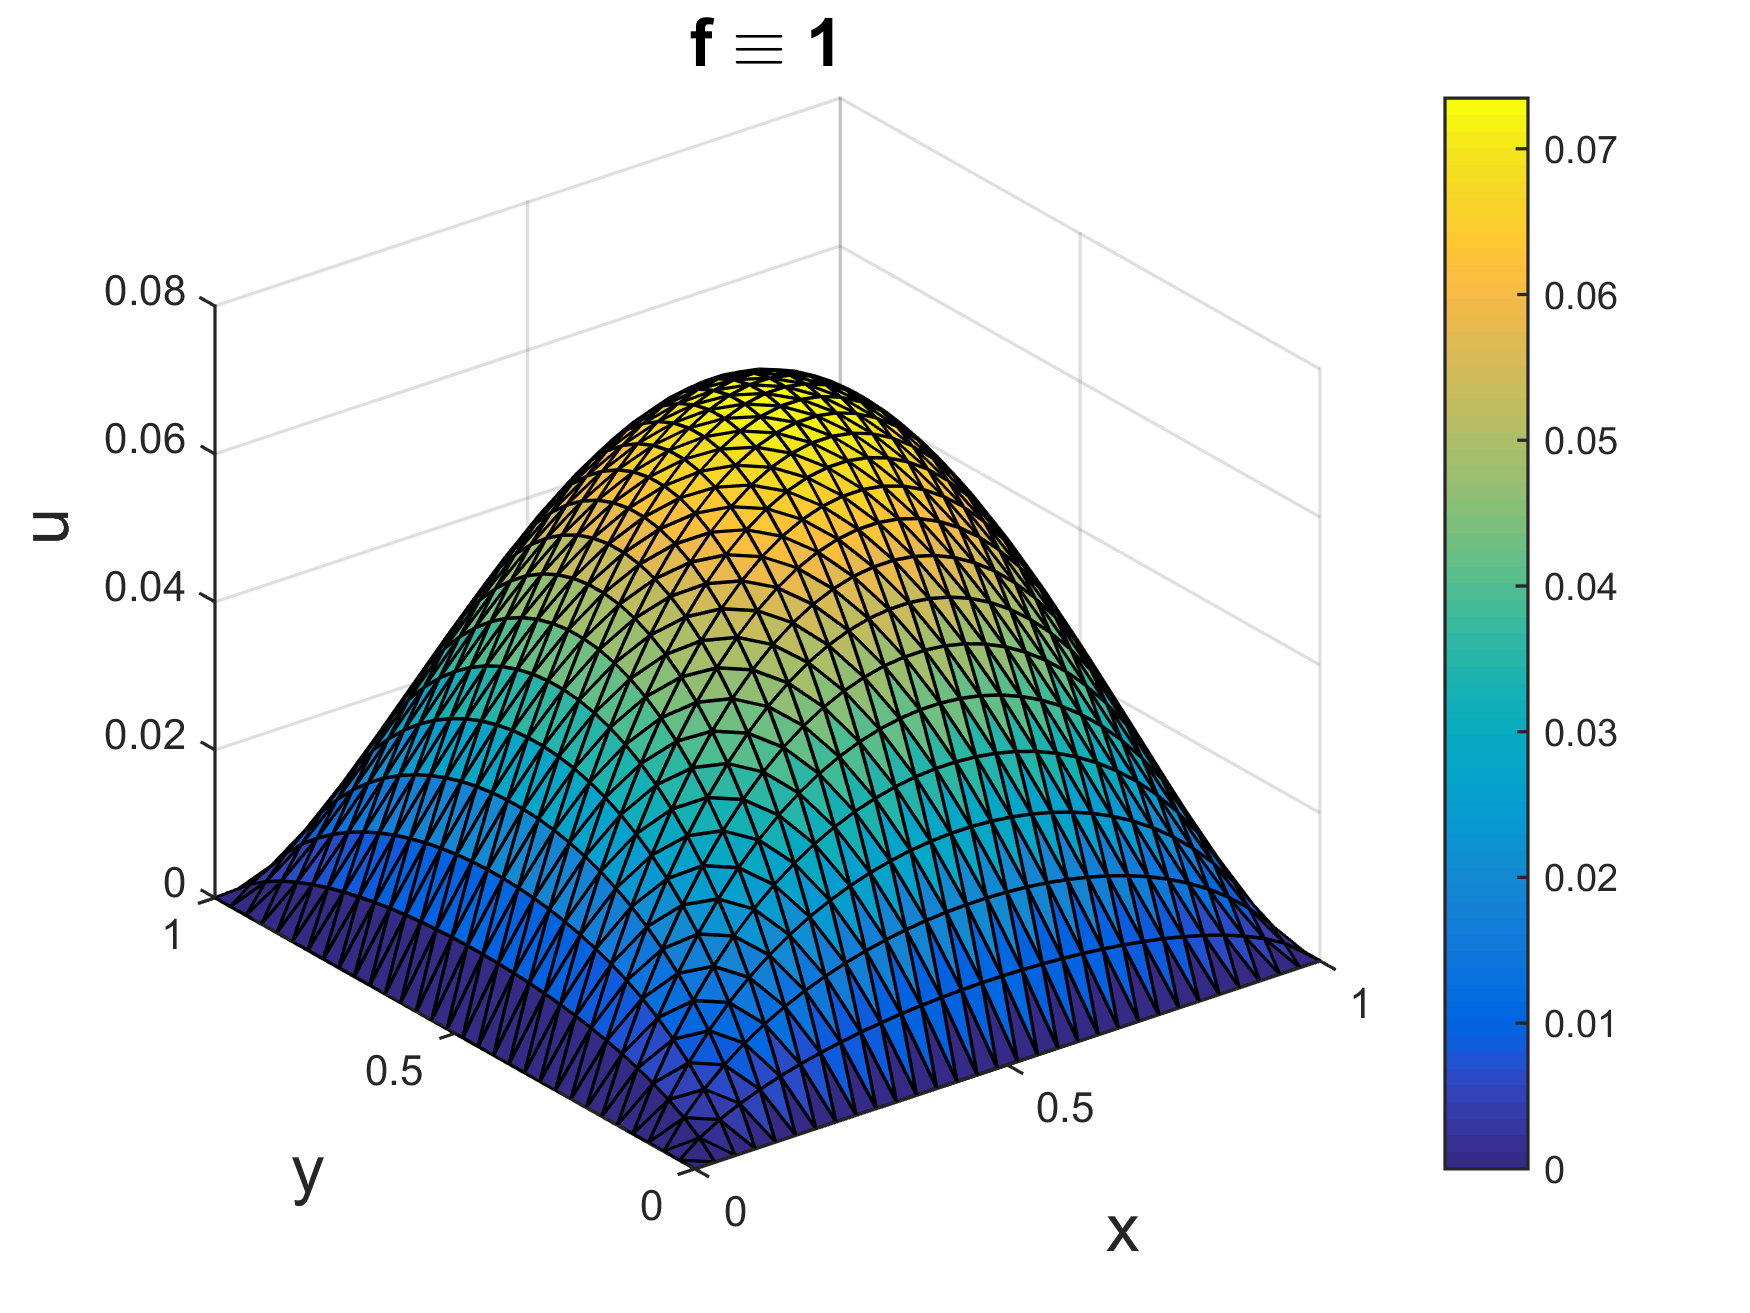
\includegraphics[width=\textwidth]{const100.png}}
		\label{fig:linu2d}
	\end{subfigure}
	~
	\begin{subfigure}{.5\textwidth}
		\centerline{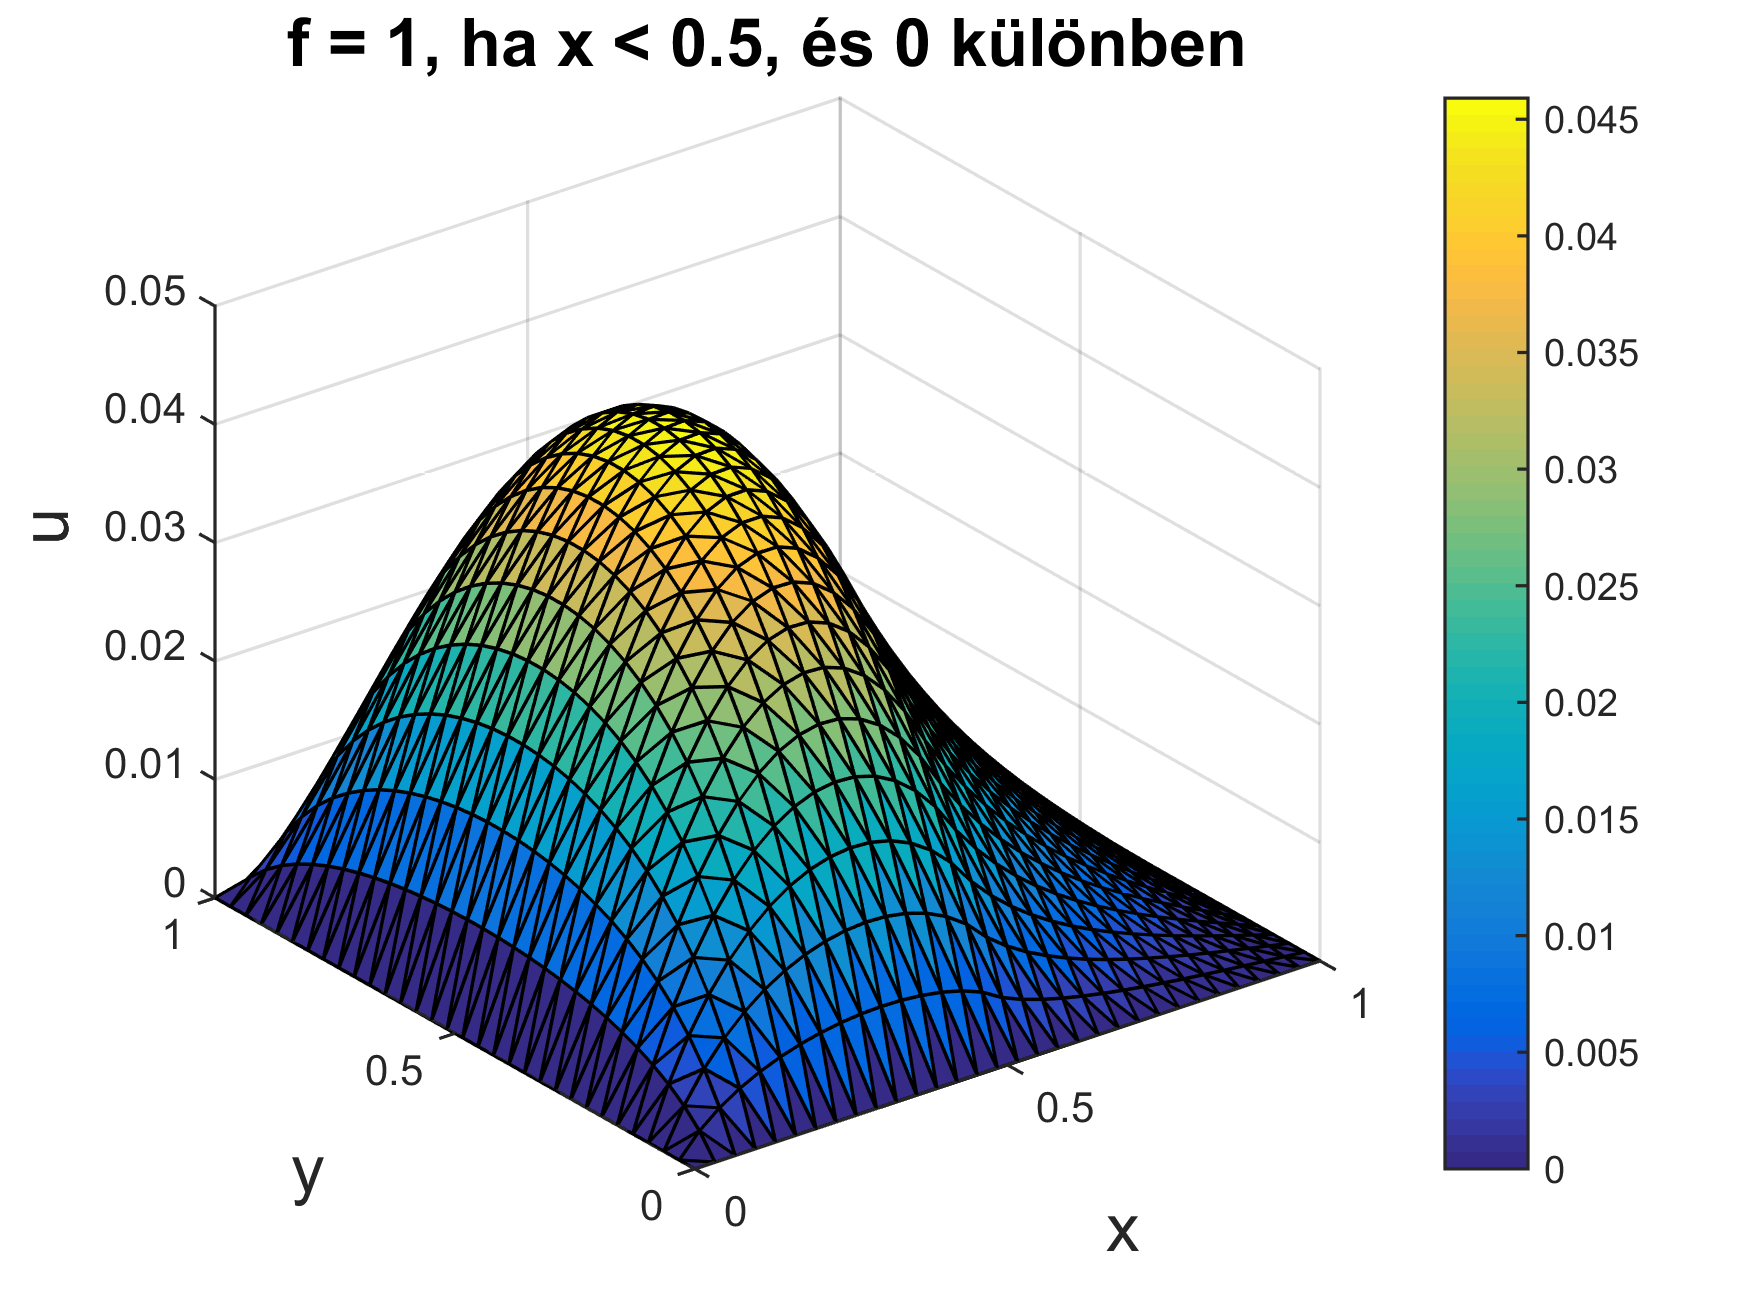
\includegraphics[width=\textwidth]{leftside50.png}}
		\label{fig:linu2d}
	\end{subfigure}
	\\
	\begin{subfigure}{.5\textwidth}
		\centerline{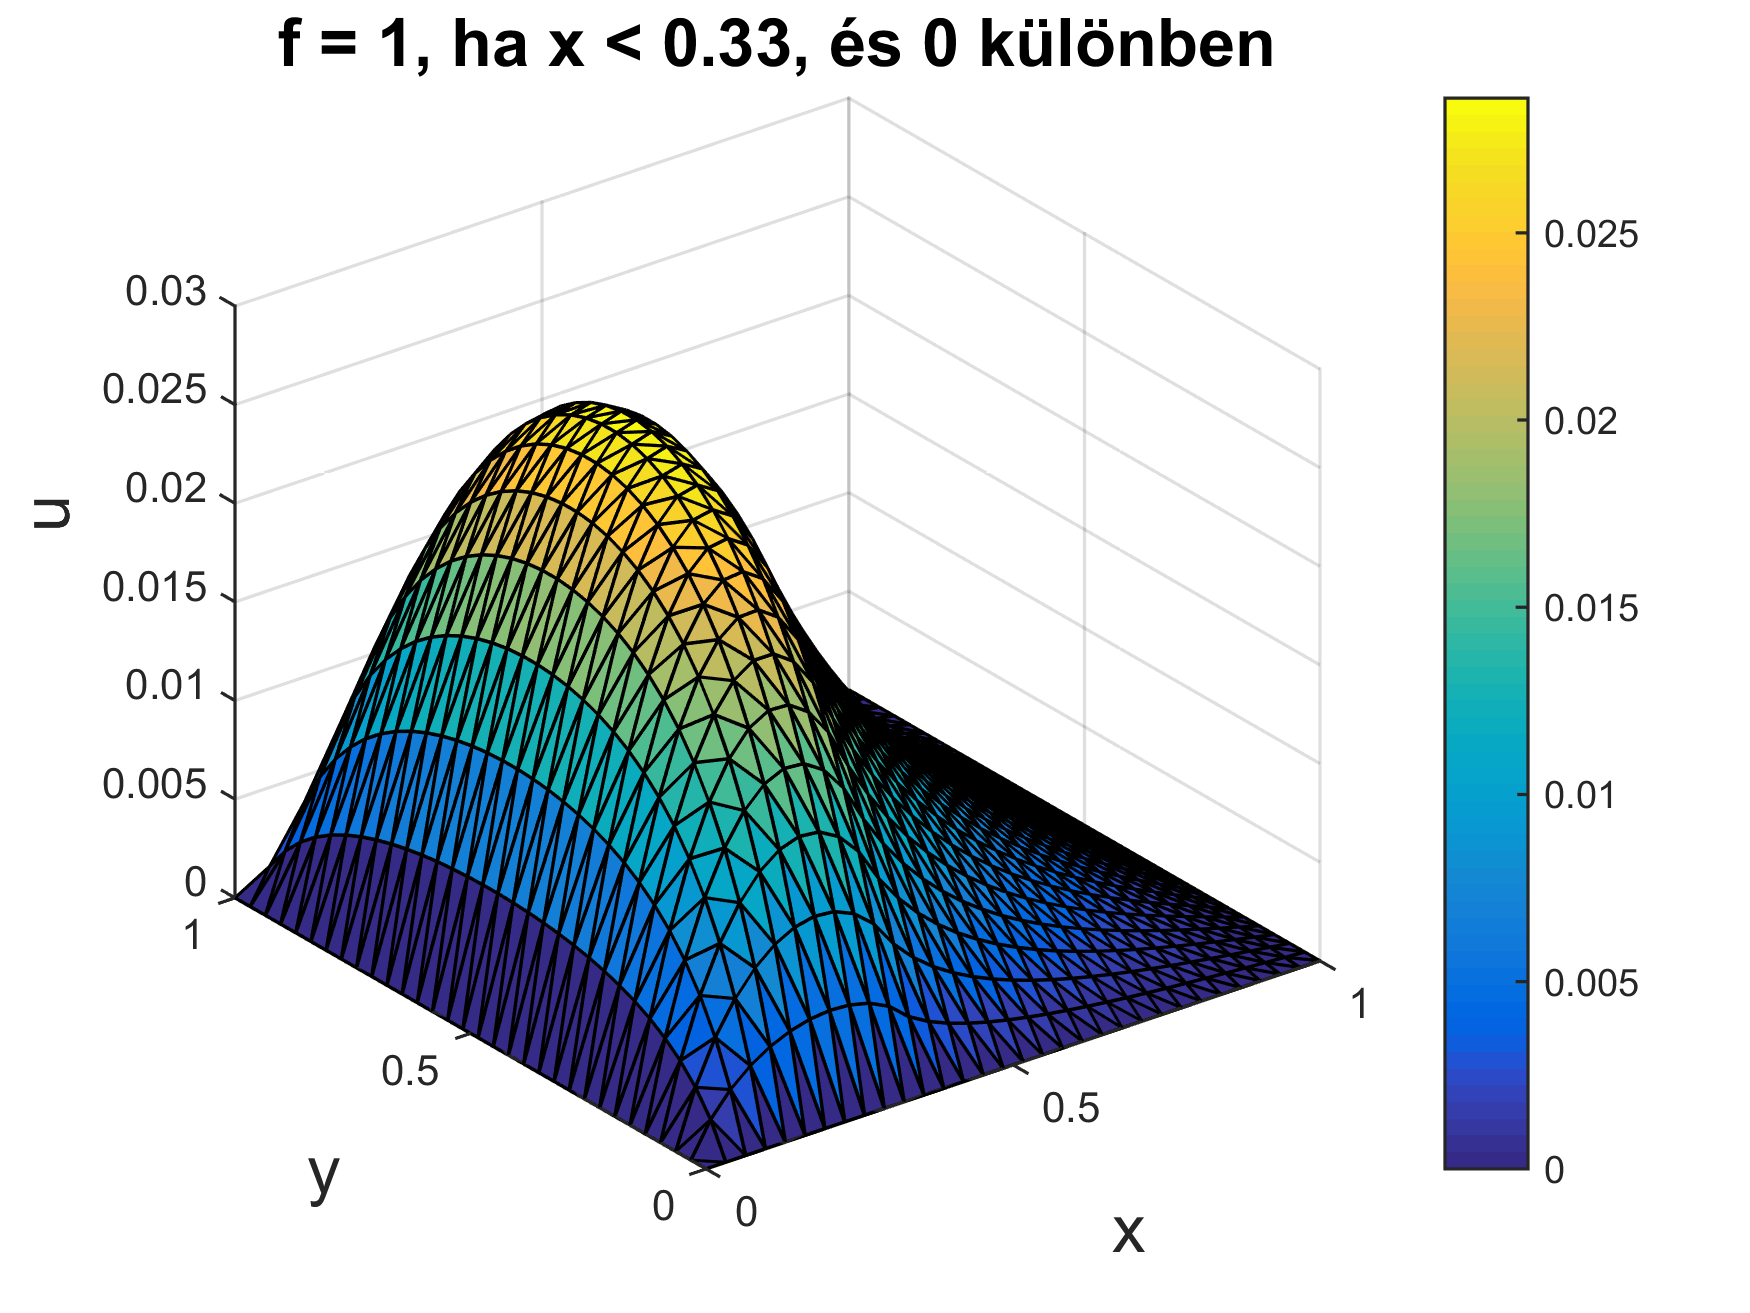
\includegraphics[width=\textwidth]{leftside33.png}}
		\label{fig:linu2d}
	\end{subfigure}
	~
	\begin{subfigure}{.5\textwidth}
		\centerline{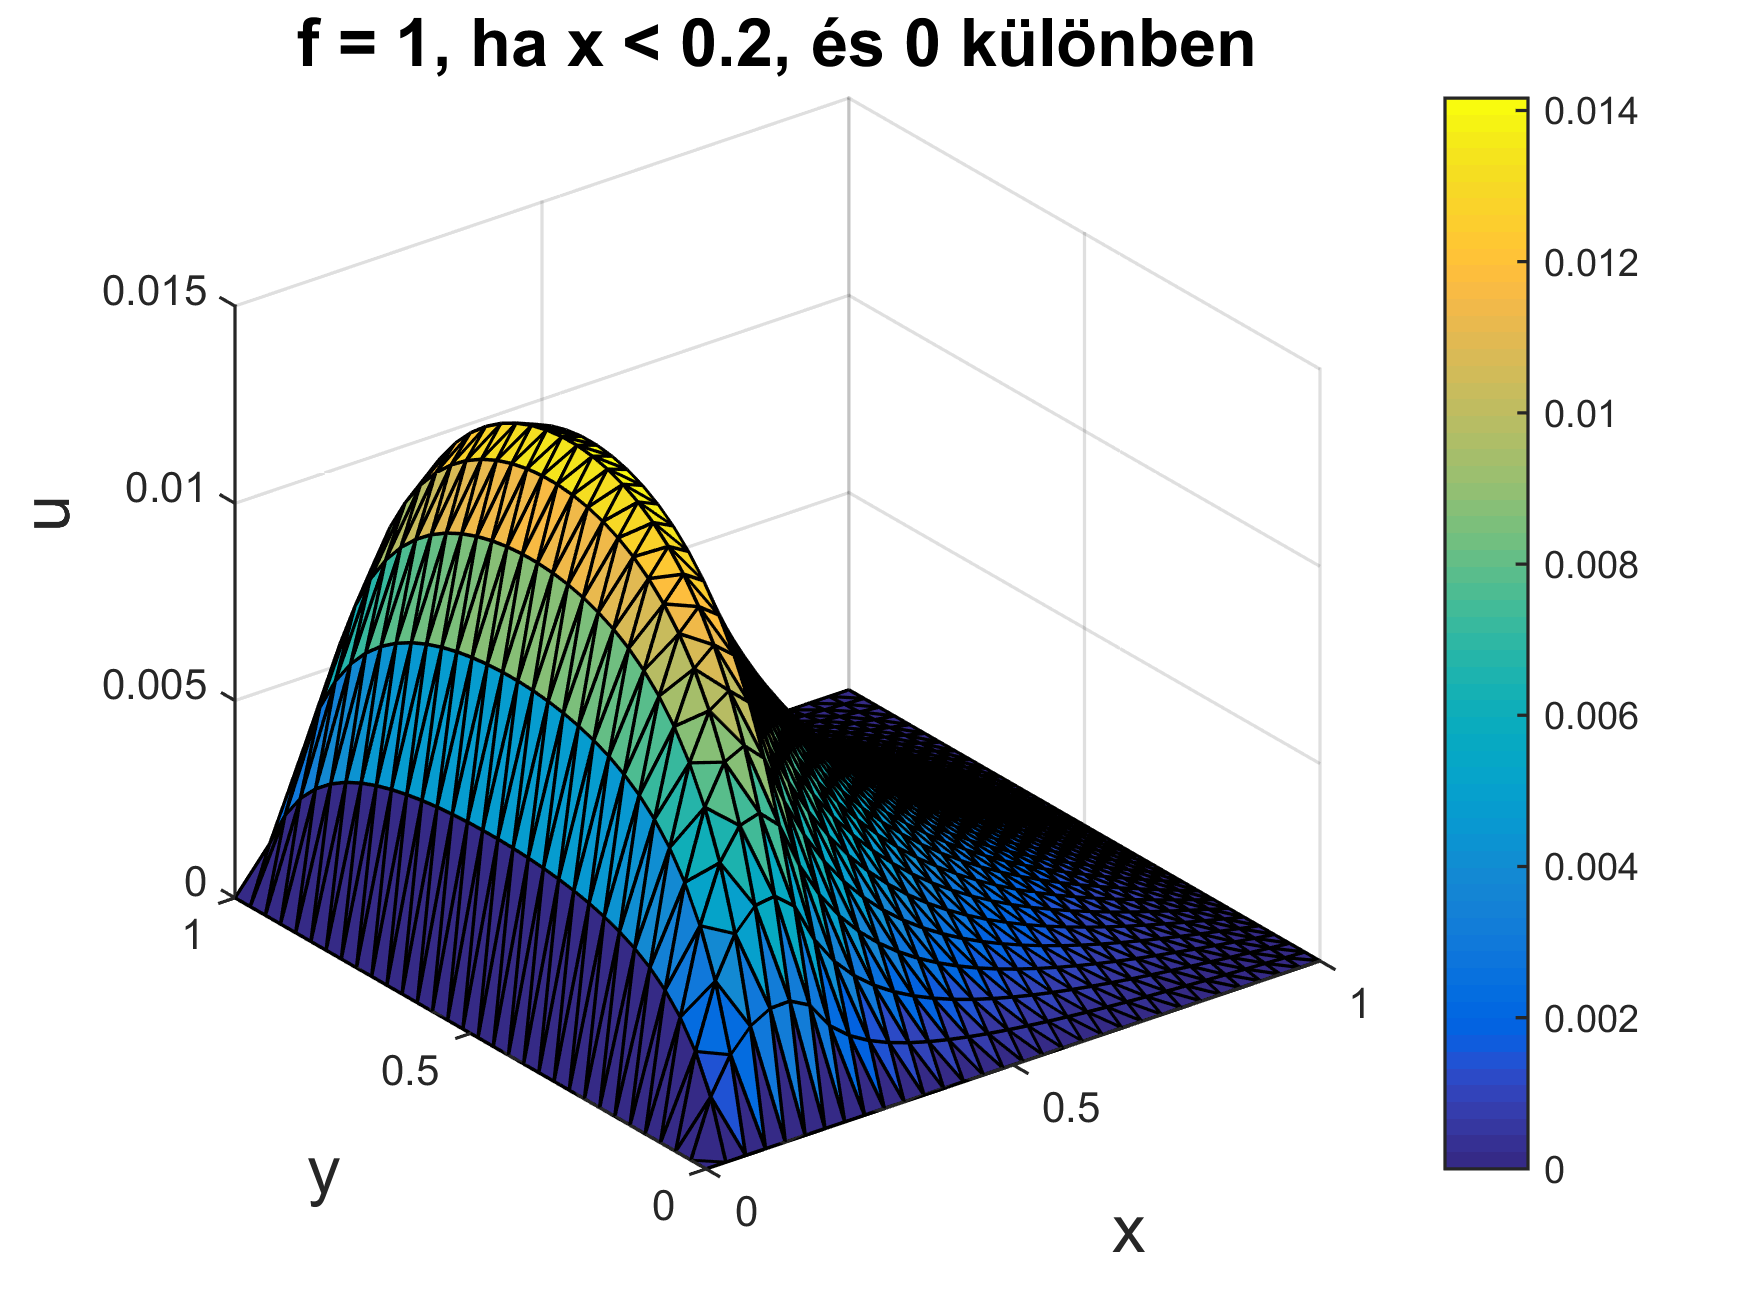
\includegraphics[width=\textwidth]{leftside20.png}}
		\label{fig:linu2d}
	\end{subfigure}
	\caption{Eredmények az $f_1$, illetve és $f_{2,k}$ jobb oldali függvényekre \eqref{f_ek_szamitashoz}, $k = 1/2, 1/3, 1/5$ mellett.}
	\label{fig:f12eredmeny}
\end{figure}

\begin{figure}[ht]
	% \centering
	\begin{subfigure}{.5\textwidth}
		\centerline{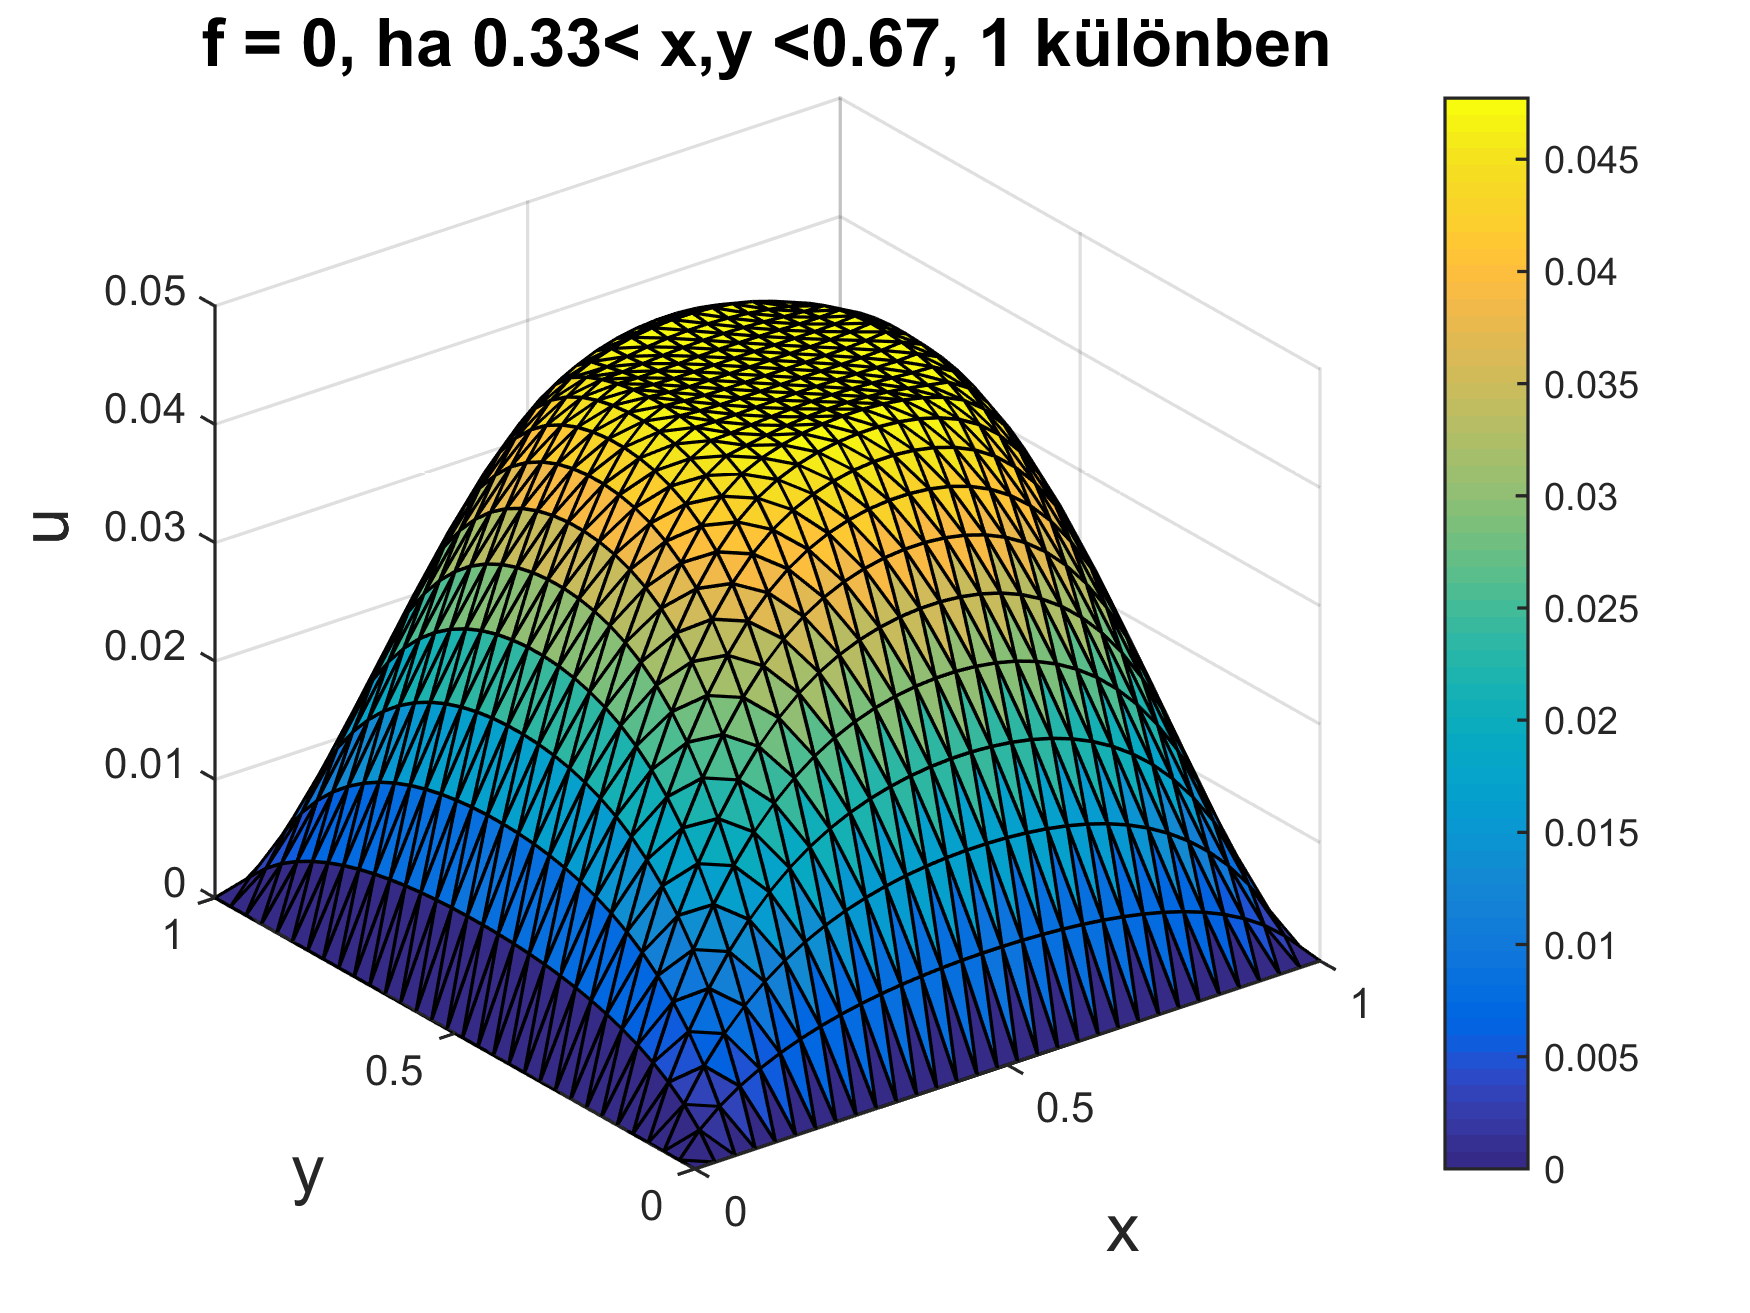
\includegraphics[width=\textwidth]{edge33.png}}
		\label{fig:linu2d}
	\end{subfigure}
	~
	\begin{subfigure}{.5\textwidth}
		\centerline{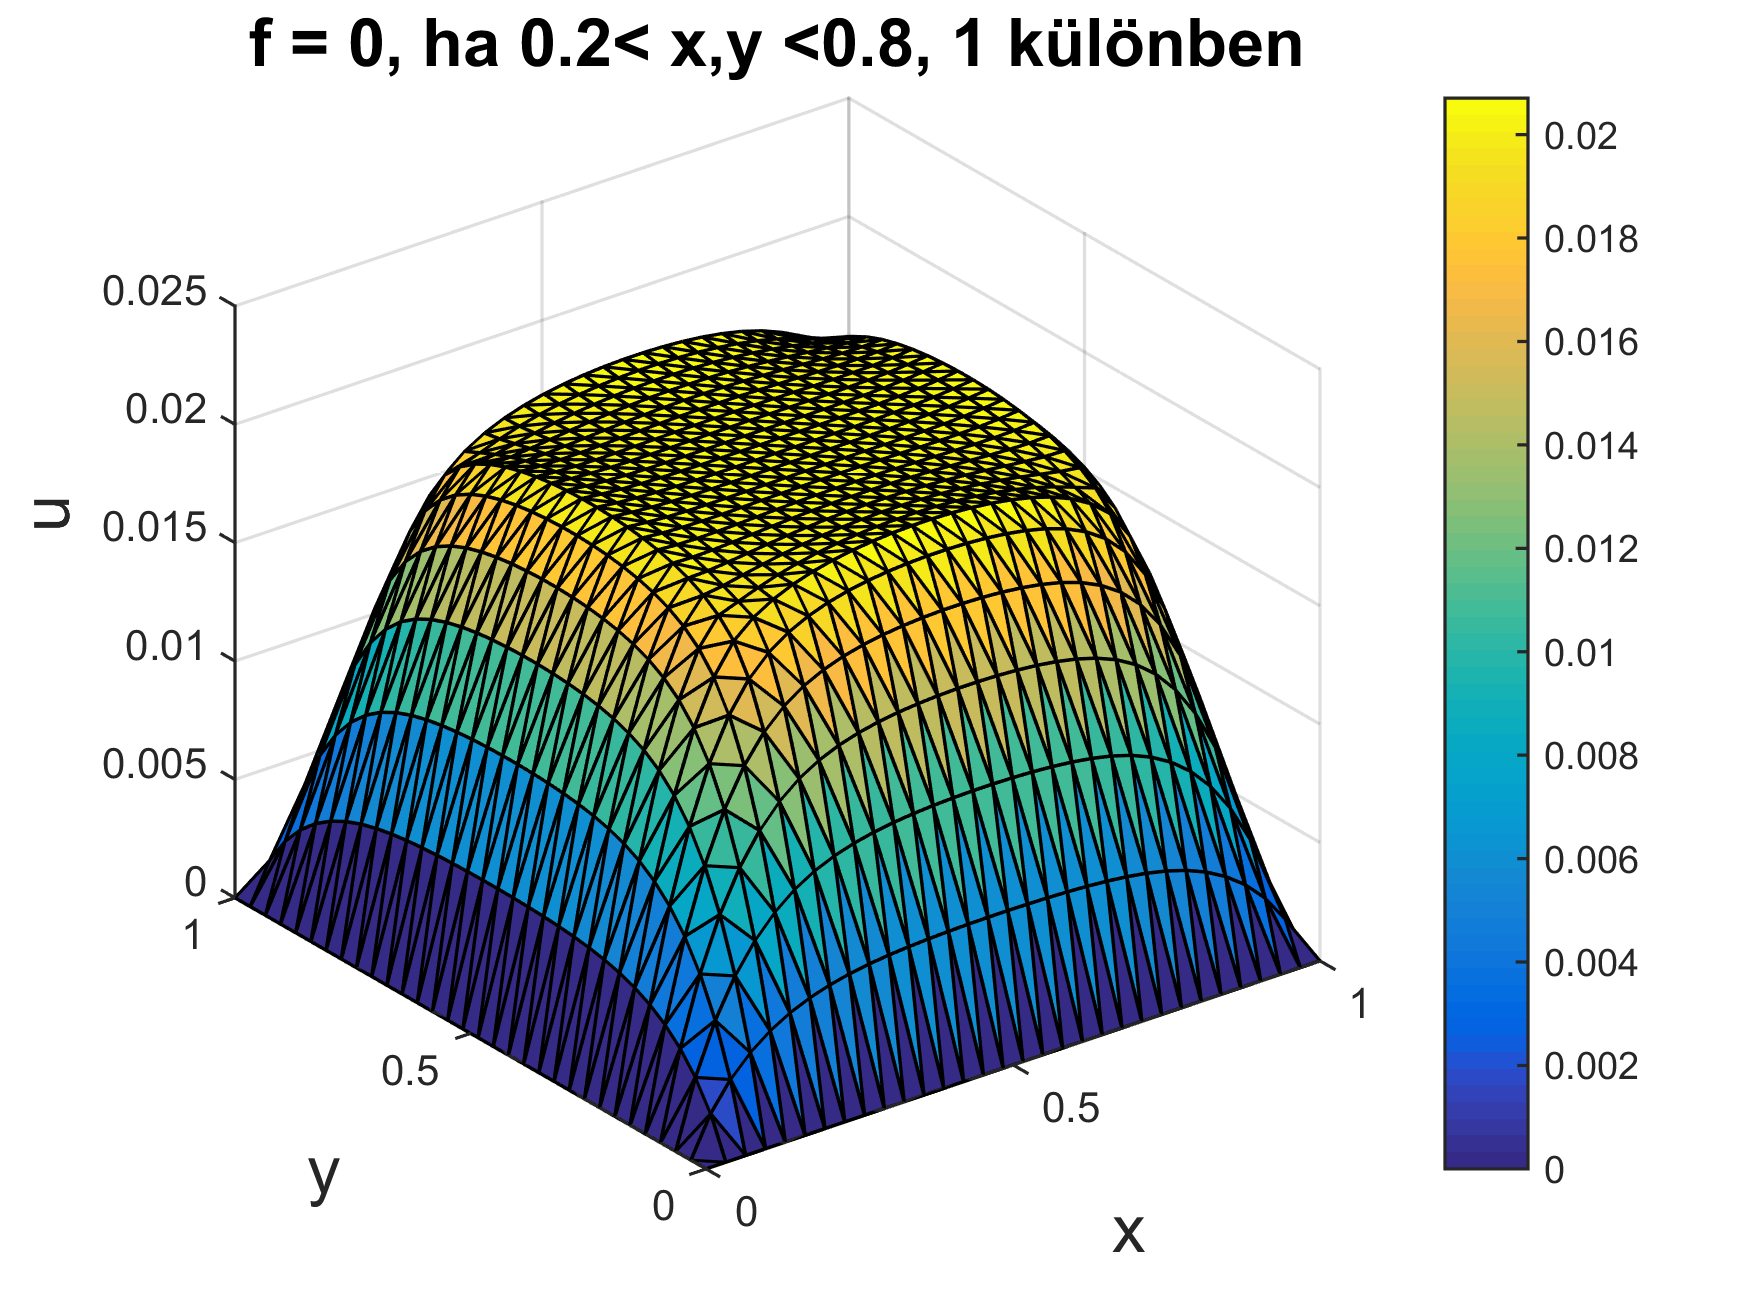
\includegraphics[width=\textwidth]{edge20.png}}
		\label{fig:linu2d}
	\end{subfigure}
	\\
	\begin{subfigure}{.5\textwidth}
		\centerline{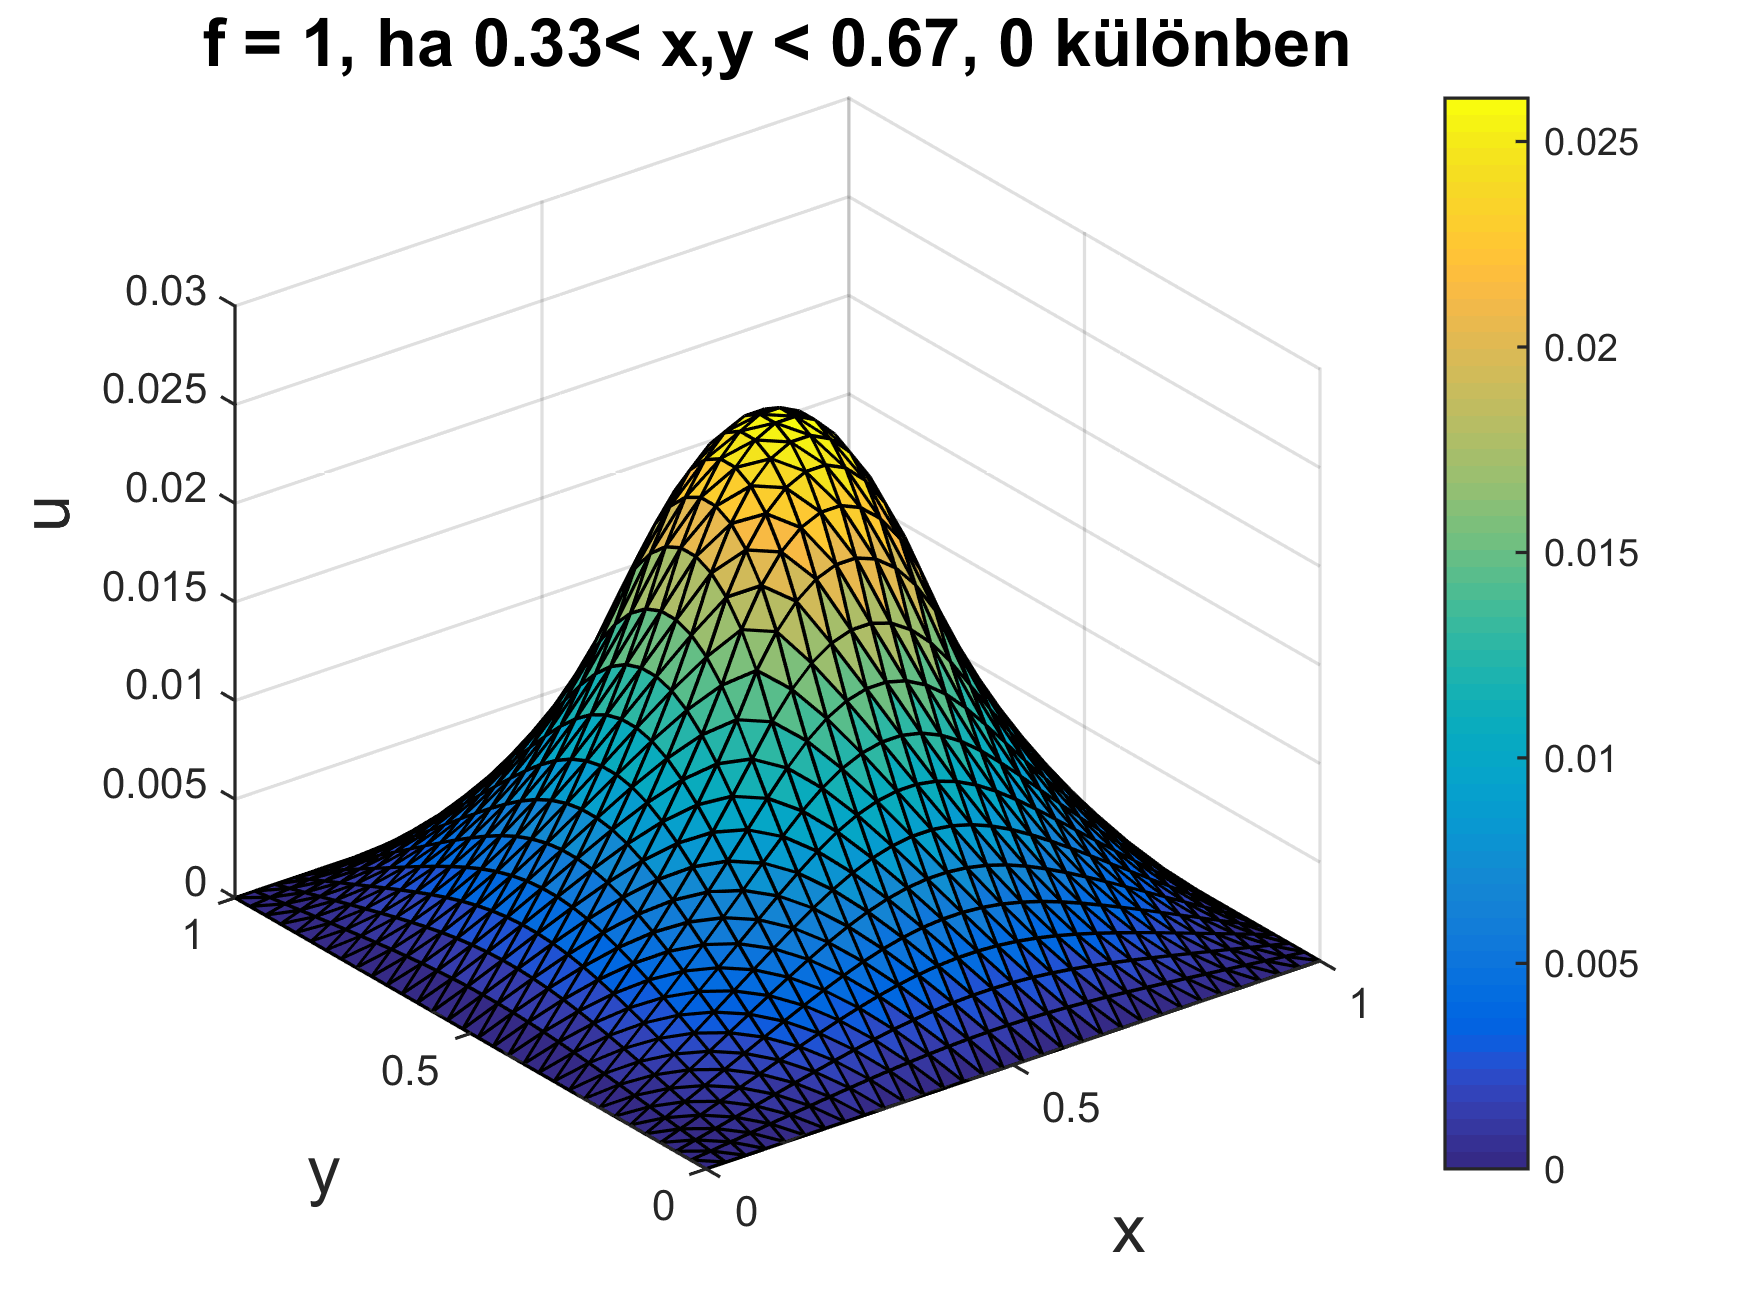
\includegraphics[width=\textwidth]{center33.png}}
		\label{fig:linu2d}
	\end{subfigure}
	~
	\begin{subfigure}{.5\textwidth}
		\centerline{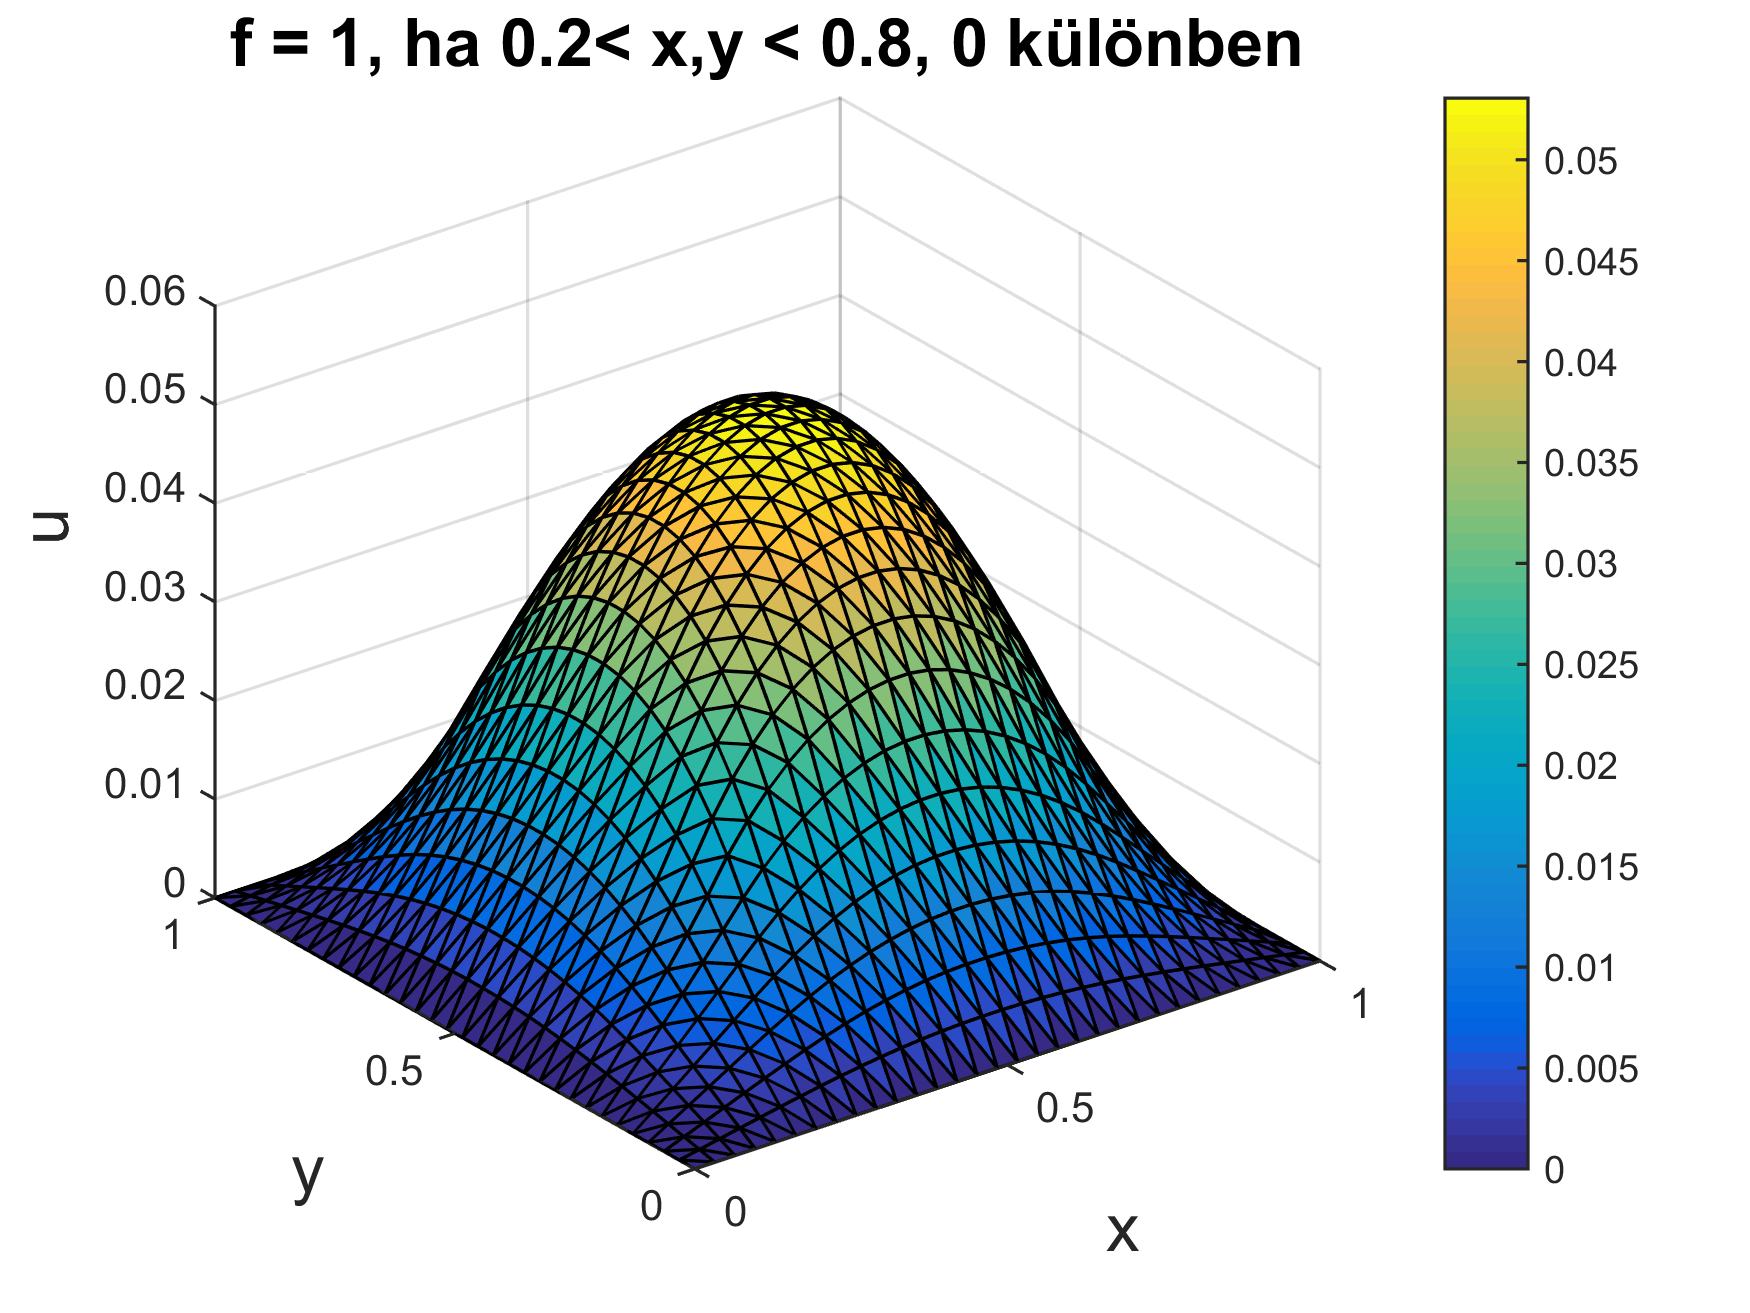
\includegraphics[width=\textwidth]{center20.png}}
		\label{fig:linu2d}
	\end{subfigure}
	\caption{Eredmények az $f_{3,k}$ és $f_{4,k}$ jobb oldali függvényekre \eqref{f_ek_szamitashoz}, $k = 1/3, 1/5$ mellett.}
	\label{fig:f34eredmeny}
\end{figure}


Az eredményekből látszik, hogy az $u_h$ végeselemes megoldás nemnegativitása mindegyik forrásfüggvény mellett teljesül. 

Az $f_{2,k}$ függvény esetében a forrás a jobb oldali $k$ szélességű sávon $1$, és a bal oldali $(1-k)$ szélességű sávon $0$. Az eredményekből látható (\ref{fig:f12eredmeny} ábra), hogy  kisebb $k$ értékek mellett a megoldás jobban megközelíti a $0$ értéket. A megoldás kovkáv felület, és kisebb $k$ értékek mellett az  $(1,y)$ szakaszon az $u_h$ gradiensvektora kisebb meredekségű.



Az $f_{3,k}$ és $f_{4,k}$ források esetében is teljesül, hogy ha a forrás kisebb területen $1$ és nagyobb részen $0$, akkor a megoldás közelebb van $0$-hoz  (\ref{fig:f34eredmeny} ábra). Az $f_{3,k}$ forráshoz tartozó megoldásoknál elmondható, hogy kisebb $k$-ra az $u_h$ a tartomány széléhez közelebb éri el maximumát. Az $f_{4,k}$ forrásra számított eredmények esetében pedig az látható, hogy kisebb $k$ értékek mellett a  széleken az $u_h$ gradiensvektora kisebb meredekségű.


\chapter*{Összefoglalás}
\addcontentsline{toc}{chapter}{Összefoglalás}  

\Aref{sec:classical_DMP}. részben ismeretetett eredmények alapján az elliptikus Dirichlet-peremmel ellátott feladatok megoldásánál, ha a megoldást lineáris végeselemekkel közelítjük, akkor ismerünk elégséges feltételeket a klasszikus diszkrét maximum-elv teljesülésére. 2 dimenziós esetben például, ha háromszögrácsot alkalmazunk, elegendő biztosítanunk, hogy a rács megfelelő finomságú és egyenletesen hegyesszögű legyen, és ha nincs a feladatban visszacsatolás, akkor a derékszögek is megengedettek. Ezek a feltételek viszonylag könnyen teljesíthetők a számítások során.

\Aref{sec:general_DMP}. szakaszban az 1 dimenziós Poisson-egyenletet vizsgáltuk. Láthattuk, hogy a klasszikus diszkrét maximum-elv nem terjeszthető ki a magasabbrendű végeselemes közelítések esetére, mert a forrásfüggvény előjele ekkor nem határozza meg a diszkrét feladat jobb oldalának előjelét. A probléma kiküszöbölésére bevezettük a diszkrét maximum-elv általánosított alakját, ami a forrásfüggvény helyett annak a végeselemes altérre vett $L^2$-vetületére szab előjelfeltételt. Ezután 1 dimenzióban megmutattuk, hogy bizonyos feltételeket kielégítő kvadratúraformulák létezése elégséges feltétele az általánosított diszkrét maximum-elv teljesülésének magasabbrendű közelítésekre.

Nyitott kérdés, hogy az általánosított diszkrét maximum-elv kiterjeszthető-e magasabb dimenzióra és általánosabb elliptikus feladatokra. Mivel a gyakorlatban van igény a magasabbrendű közelítések alkalmazására, fontos lenne a maximum-elv kiterjeszthetőségének vizsgálata. 

\chapter*{Köszönetnyilvánítás}
\addcontentsline{toc}{chapter}{Köszönetnyilvánítás}

Ezúton köszönetet mondani konzulensemnek, Karátson Jánosnak a segítségéért, türelméért, és hogy munkámat alaposan és kritikusan ellenőrizte. 

Továbbá szeretném megköszönni családomnak és barátaimnak a szakszerű hibaellenőrzést, valamint a rengeteg támogatást, amit képzésem ideje alatt kaptam tőlük.


% \appendix
% \chapter{A futtatásokhoz tartozó MATLAB fájlok}\label{matlabkodok}
\chapter*{Függelék}\label{fuggelek}
\addcontentsline{toc}{chapter}{Függelék}  

\section*{A futtatásokhoz tartozó MATLAB fájlok}\label{matlabkodok}
\addcontentsline{toc}{section}{A futtatásokhoz tartozó MATLAB fájlok} 

\lstinputlisting{\matlabpath/solve_2DPoi_for_multiple_rhs_utf8.m"}
\lstinputlisting{\matlabpath/FEM_2DPoissonHomogenousDirichlet_utf8.m"}







\begin{thebibliography}{9}
	
	\bibitem{pdnm}
		Horváth Róbert, Izsák Ferenc, Karátson János. Parciális differenciálegyenletek numerikus módszerei számítógépes alkalmazásokkal. Elektronikus jegyzet, Eötvös Loránd Tudományegyetem, 2013.

	\bibitem{kar-kor}
		J. Karátson, S. Korotov. Discrete maximum principles for finite element solutions of nonlinear elliptic problems with mixed boundary conditions. Numer. Math., 99: 669–698, 2005.

	\bibitem{besenyei} 
		Besenyei Ádám, Komornik Vilmos, Simon László. Parciális differenciálegyenletek. Elektronikus jegyzet, Typotex, 2013.
	 
	\bibitem{ciarlet-raviart}
		 P. G. Ciarlet, P. A. Raviart. Maximum principle and uniform convergence for the finite element method. Comput. Methods Appl. Mech. Engrg., 2: 17–31, 1973.

	\bibitem{sol-vej}
		Pavel Šolín, Tomáš Vejchodský. A weak discrete maximum principle for hp-FEM. Journal of Computational and Applied Mathematics, 209: 54–65, 2007.

	\bibitem{sol-seg}
		P. Šolín, K. Segeth, I. Doležel. Higher-order Finite Element Methods. Chapman \& Hall/CRC Press, Boca Raton, 2003.
		
	\bibitem{gilbarg}
		D. Gilbarg, N. S. Trudinger. Elliptic Partial Differential Equations of Second Order. Springer, Berlin - Heidelberg - New York - Barcelona - Hong Kong - London - Milan - Paris - Singapore - Tokyo, 2001.

	\bibitem{stoyan2}
		Stoyan Gisbert, Takó Galina. Numerikus módszerek 2. ELTE - Typotex, Budapest, 1995.
	
	\bibitem{stoyan3}
		Stoyan Gisbert, Takó Galina. Numerikus módszerek 3. ELTE - Typotex, Budapest, 1997.
		
	
	\bibitem{numfunk} 
		Karátson János. Numerikus funkcionálanalízis. Elektronikus jegyzet, Typotex, 2013.	
		
	\bibitem{varga}
		R. Varga. Matrix iterative analysis. Prentice Hall, New Jersey, 1962.
		
		
	
\end{thebibliography}



\end{document}